\chapter{数论算法 (Algorithms with numbers)}

本章的核心主线之一，是两个初看极为相似的古老问题之间形成的鲜明对比：
\begin{itemize}
    \item \textbf{质因数分解 (FACTORING)}：给定一个正整数 $N$，将其表示为质因子的乘积。
    \item \textbf{素性测试 (PRIMALITY)}：给定一个正整数 $N$，判断它是否为一个素数（质数）。
\end{itemize}

质因数分解极其困难。尽管几个世纪以来世界上最聪明的数学家和计算机科学家付出了巨大努力，目前已知用于分解一个数 $N$ 的最快方法所需的时间仍然是 $N$ 的二进制位数的指数级别。

然而，我们很快就会看到，判断 $N$ 是否为素数却可以高效地完成！更引人入胜的是，这两个紧密关联的问题之间这种奇特的悬殊差距——一个极难，另一个极易——构成了保障当今全球信息环境中安全通信的核心技术基石。

为了领会这些深刻洞见，我们首先需要为一系列涉及数字的计算任务设计算法。我们从基础算术开始，这是一个绝佳的起点，因为众所周知，“算法”（algorithms）一词最初指代的就是解决这些四则运算问题的方法。

\section{基础算术 (Basic arithmetic)}

\subsection{加法 (Addition)}
我们在年幼时就学习了标准的加法法则，以至于很少会去思考它为什么有效。现在让我们重温这一过程并仔细审视。

十进制数具有一个基本性质：
\begin{center}
    \textbf{任意三个单数字（0--9）相加之和最多只有两位数。}
\end{center}
快速验算一下：其最大和为 $9 + 9 + 9 = 27$，确实只有两位。事实上，这一法则不仅在十进制下成立，在任何基数（进制）$b \ge 2$ 下都成立（参见习题 1.1）。例如在二进制中，三个单比特数字的最大可能和为 $1 + 1 + 1 = 3 = 11_2$，也是一个 2 比特数字。

\begin{sidebarbox}{进位制与对数 (Bases and logs)}
自然，数字 10 并没有什么特别之处——我们只是恰好有 10 根手指，因此 10 成为了停顿并将计数提升至更高阶层次的天然选择。玛雅人基于数字 20 发展了一套类似的位值制记数系统（看来他们不穿鞋，对吧？）。当然，今天的计算机使用二进制来表示数字。

在以 $b$ 为底的进位制中，表示非负整数 $N \ge 0$ 需要多少位数字？我们来看一下——在以 $b$ 为底的进制中，用 $k$ 位数字可以表示最大到 $b^k - 1$ 的数；例如在十进制中，三位数字最多可以表示到 $999 = 10^3 - 1$。通过反解 $k$，我们发现以 $b$ 为底表示 $N$ 需要 $\lceil \log_b (N + 1) \rceil$ 位数字（大约是 $\log_b N$ 位，上下浮动不超过 1 位）。

当我们改变进位制时，一个数字的大小（位数）会发生怎样的变化？回忆换底公式：$\log_b N = (\log_a N) / (\log_a b)$。因此，整数 $N$ 在底数 $a$ 下的位数等于其在底数 $b$ 下的位数乘以一个常数因子 $\log_a b$。因此，在大 $O$ 记号下，进位制的底数是无关紧要的，我们直接将其位数简写为 $O(\log N)$。当我们不显式指明底数时（我们几乎绝不指明），默认指的是以 2 为底的对数 $\log_2 N$。

顺便提一句，函数 $\log N$ 在我们的学科中反复出现，且具有多种化身。以下是一些例子：
\begin{enumerate}
    \item $\log N$ 当然是 2 为了得到 $N$ 所必须提升的幂次（指数）。
    \item 反向来看，它也可以被视为将 $N$ 连续折半直至变为 1 所需的次数（更准确地说是 $\lfloor \log N \rfloor$）。当一个算法在每次迭代中都将数字减半时，这一点非常有用，本章稍后的几个例子中就会看到。
    \item 它是 $N$ 在二进制表示中的比特数（更准确地说是 $\lfloor \log(N + 1) \rfloor$）。
    \item 它也是拥有 $N$ 个节点的完全二叉树的深度（更准确地说是 $\lceil \log N \rceil$）。
    \item 它甚至在相差一个常数因子的意义下等于调和级数和 $1 + \frac{1}{2} + \frac{1}{3} + \cdots + \frac{1}{N}$（参见习题 1.5）。
\end{enumerate}
\end{sidebarbox}

这个简单的性质为我们在任意进位制下相加两个数提供了方法：将它们的右端（低位）对齐，然后执行一次自右向左的遍历，逐位计算和，并将溢出保留为进位。因为我们知道每次单独相加的和最多只有两位数，所以进位始终是一个单数字；因此在任意给定步骤中，都只需将三个单数字相加。下面给出了二进制下计算 $53 + 35$ 的示例：

\begin{center}
\begin{tabular}{rcccccccl}
进位 (Carry): & \textcolor{blue}{1} & \textcolor{blue}{1} & \textcolor{blue}{1} & \textcolor{blue}{1} & & & \\
& & 1 & 1 & 0 & 1 & 0 & 1 & (53) \\
$+$ & & 1 & 0 & 0 & 0 & 1 & 1 & (35) \\
\hline
& 1 & 0 & 1 & 1 & 0 & 0 & 0 & (88)
\end{tabular}
\end{center}

通常我们会用伪代码详细写出算法，但在当前情况下该算法如此常见，我们不再赘述其伪代码，而是直接进入对其效率的分析。

给定两个二进制数 $x$ 和 $y$，我们的加法算法需要花费多长时间？这是贯穿全书我们将持续提出的核心问题。我们希望将答案表示为输入规模（即 $x$ 和 $y$ 的比特数，或者说键盘输入它们所需的按键次数）的函数。

假设 $x$ 和 $y$ 各自都是 $n$ 位长；在本章中，我们将始终使用字母 $n$ 来表示数字的位数。那么 $x$ 与 $y$ 之和最多为 $n + 1$ 位，并且该和的每一个单独比特位都可以在常数时间内计算完成。因此，加法算法的总运行时间具有 $c_0 + c_1 n$ 的形式（其中 $c_0$ 和 $c_1$ 为某常数）；换句话说，它是线性的。我们无需过分关注 $c_0$ 和 $c_1$ 的具体精确值，而是着眼于大局，将运行时间记为 $O(n)$。

既然我们有了一个已知运行时间的可行算法，我们的思维便不可避免地转向：是否存在更好的算法？

是否存在更快的算法？（这是另一个贯穿始终的问题）。对于加法而言，答案很简单：为了将两个 $n$ 位的数字相加，我们至少必须读入它们并写下答案，而仅仅这两项操作就需要 $n$ 步基本操作。因此，在不计乘法常数因子的意义下，该加法算法已经是最优的！

有些读者在此可能会感到困惑：为什么是 $O(n)$ 次操作？今天的计算机不是一条指令就能完成二进制加法吗？这里有两个回答。首先，对于位数在当今计算机字长范围之内（例如 32 位或 64 位）的整数，确实可以在单条机器指令中完成加法。但是，正如本章稍后将变得显而易见的那样，在实际应用中经常需要处理远大于此的数字（可能长达数千位）。在真实计算机上对如此巨大的数字进行加法和乘法，本质上就是逐比特位地执行操作。其次，当我们旨在理解算法时，研究那些编码在当今计算机硬件底层的基本算法也是极具意义的。在做这些分析时，我们将重点关注算法的\textbf{比特复杂度}（bit complexity），即对单个比特执行的基本操作次数——因为这种核算方式直接反映了实现该算法所需的硬件资源（晶体管和布线）数量。

\subsection{乘法与除法 (Multiplication and division)}
接下来讨论乘法！小学学到的乘法算法是为两个数 $x$ 和 $y$ 创建一个中间和数组，其中每一项代表 $x$ 与 $y$ 的某单个数字的乘积。这些值经过适当的左移，然后全部相加。假设我们要计算 $13 \times 11$，用二进制表示即 $x = 1101_2$ 且 $y = 1011_2$。乘法过程如下进行：

\begin{center}
\begin{tabular}{rccccccccl}
& & & & 1 & 1 & 0 & 1 & & ($x = 13$) \\
$\times$ & & & & 1 & 0 & 1 & 1 & & ($y = 11$) \\
\hline
& & & & 1 & 1 & 0 & 1 & & ($1101 \times 1$) \\
& & & 1 & 1 & 0 & 1 & & & ($1101 \times 1$，左移1位) \\
& & 0 & 0 & 0 & 0 & & & & ($1101 \times 0$，左移2位) \\
$+$ & 1 & 1 & 0 & 1 & & & & & ($1101 \times 1$，左移3位) \\
\hline
& 1 & 0 & 0 & 0 & 1 & 1 & 1 & 1 & (二进制 143)
\end{tabular}
\end{center}

在二进制中这一过程尤其简单，因为每一行中间结果要么全为零，要么就是 $x$ 本身经过相应位数的左移。同时请注意，左移恰好是以进位制基数（这里是 2）为乘数的快捷乘法。（类似地，右移的效果是除以基数，并在必要时向下取整。）

该乘法过程的正确性证明见习题 1.6；我们继续计算它所需的时间。如果 $x$ 和 $y$ 均为 $n$ 位长，则存在 $n$ 个中间行，考虑到移位，每行的长度最多为 $2n$ 位。将这 $n$ 行逐次两两相加的总时间为：
\[
\underbrace{O(n) + O(n) + \cdots + O(n)}_{n-1 \text{ 次}} = O(n^2),
\]
这是输入规模的二次方（quadratic）：虽然仍是多项式时间，但比起加法要慢得多（正如我们所有人从小学起就隐约感觉到的那样）。

但阿尔·花拉子米（Al Khwarizmi）知道另一种乘法方法，该方法至今在一些欧洲国家仍有使用。为了相乘两个十进制数 $x$ 和 $y$，将它们并排写下，如下例所示。然后重复以下步骤：将第一个数除以 2 并向下取整（如果为奇数则舍去 0.5），同时将第二个数翻倍。持续进行直到第一个数变为 1。然后划掉第一个数为偶数的所有行，并将第二列中剩余的数全部相加。

\begin{center}
\begin{tabular}{rrll}
11 & 13 & & \\
5 & 26 & & \\
2 & 52 & (划掉) & \\
1 & 104 & & \\
\hline
& \textbf{143} & (答案: $13 + 26 + 104 = 143$) &
\end{tabular}
\end{center}

如果我们对比这两种算法——二进制乘法与乘数连续折半乘法，会惊奇地发现它们做的事情完全相同！在第二种算法中所累加的三个数字，恰恰就是二进制方法中将 13 乘以 2 的幂次所得到的项。只不过这一次 11 并没有直接以二进制形式给出，我们通过对它连续除以 2 得到的数的奇偶性，动态提取出了它的二进制表示。阿尔·花拉子米的第二种算法是十进制与二进制的奇妙结合！

因此，同一算法可以有不同的包装方式。为了展现多样性，我们采用第三种表述形式——图 \ref{fig:mult_recursive} 中的递归算法，它直接实现了如下递推规则：
\[
x \cdot y = \begin{cases}
2 \cdot (x \cdot \lfloor y / 2 \rfloor), & \text{若 } y \text{ 为偶数} \\
x + 2 \cdot (x \cdot \lfloor y / 2 \rfloor), & \text{若 } y \text{ 为奇数}.
\end{cases}
\]

\begin{figure}[htbp]
\centering
\begin{tcolorbox}[colback=white,colframe=gray!50!black,title={\textbf{图 1.1}\quad 法式乘法 (Multiplication à la Française)}]
\begin{algorithmic}[1]
\Function{multiply}{$x, y$}
    \State \textbf{Input:} 两个 $n$ 位整数 $x$ 和 $y$，其中 $y \ge 0$
    \State \textbf{Output:} 它们的乘积
    \If{$y = 0$} \Return $0$ \EndIf
    \State $z = \Call{multiply}{x, \lfloor y/2 \rfloor}$
    \If{$y \text{ 为偶数}$}
        \State \Return $2z$
    \Else
        \State \Return $x + 2z$
    \EndIf
\EndFunction
\end{algorithmic}
\end{tcolorbox}
\label{fig:mult_recursive}
\end{figure}

该算法是否正确？上述递归规则显而易见是正确的；因此验证算法的正确性仅仅在于确认它忠实地模拟了该规则并正确处理了基本情况（$y = 0$）。

该算法需要多长时间？它必然在 $n$ 次递归调用后终止，因为每次调用中 $y$ 都减半——即其二进制位数减少了 1 位。而每次递归调用中包含这些操作：一次除以 2（右移）；一次奇偶性测试（查看最低有效位）；一次乘以 2（左移）；以及至多一次加法，共计 $O(n)$ 次比特操作。因此总耗时为 $O(n^2)$，与之前完全一致。

我们能否做得更好？直观上，乘法似乎需要将其中一个输入的约 $n$ 个倍数相加，而我们知道每次加法是线性的，因此 $n^2$ 次比特操作似乎不可避免。然而令人惊叹的是，在第 2 章中我们将会看到，我们可以做得显著更好！

接下来是除法。将一个整数 $x$ 除以另一个非零整数 $y \ne 0$，意味着要找到商 $q$ 和余数 $r$，满足 $x = yq + r$ 且 $0 \le r < y$。我们在图 \ref{fig:div_recursive} 中给出了除法的递归版本；与乘法类似，它也需要二次方时间。对该算法的严谨分析见习题 1.8。

\begin{figure}[htbp]
\centering
\begin{tcolorbox}[colback=white,colframe=gray!50!black,title={\textbf{图 1.2}\quad 除法 (Division)}]
\begin{algorithmic}[1]
\Function{divide}{$x, y$}
    \State \textbf{Input:} 两个 $n$ 位整数 $x$ 和 $y$，其中 $y \ge 1$
    \State \textbf{Output:} $x$ 除以 $y$ 的商与余数 $(q, r)$
    \If{$x = 0$} \Return $(q, r) = (0, 0)$ \EndIf
    \State $(q, r) = \Call{divide}{\lfloor x/2 \rfloor, y}$
    \State $q = 2 \cdot q,\; r = 2 \cdot r$
    \If{$x \text{ 为奇数}$} $r = r + 1$ \EndIf
    \If{$r \ge y$} $r = r - y,\; q = q + 1$ \EndIf
    \State \Return $(q, r)$
\EndFunction
\end{algorithmic}
\end{tcolorbox}
\label{fig:div_recursive}
\end{figure}

\section{模算术 (Modular arithmetic)}

随着反复的加法或乘法，数字可能会变得极其庞大繁琐。幸运的是，在日常生活中，当时间达到 24 点时我们会将其重置为 0，每过 12 个月月份又会重归一月。类似地，对于计算机处理器的内置算术运算，数字通常被限制在某一固定大小（例如 32 位），这对于大多数应用场景已经被认为足够宽裕。

但对于我们即将迈向的应用——素性测试与密码学——我们需要处理显著大于 32 位的数字，但这些数字的取值范围却仍然受到限制。

模算术（同余算术）就是一种处理有限范围整数的系统。我们定义 $x \bmod N$ 为 $x$ 除以 $N$ 所得的余数；即若 $x = qN + r$ 且 $0 \le r < N$，则 $x \bmod N = r$。这赋予了数字之间一种增强的等价概念：若 $x$ 和 $y$ 之差是 $N$ 的倍数，则称它们模 $N$ 同余，记作：
\[
x \equiv y \pmod N \iff N \mid (x - y).
\]
例如，$253 \equiv 13 \pmod{60}$，因为 $253 - 13$ 是 60 的倍数；在日常生活中更通俗的表述是，253 分钟等于 4 小时零 13 分钟。这些数字也可以是负数，例如 $59 \equiv -1 \pmod{60}$：当某一小时过了 59 分钟时，也就是距离下一小时还差 1 分钟。

\begin{figure}[htbp]
\centering
\begin{tikzpicture}[scale=0.85]
    \draw[thick] (0,0) circle (1.8cm);
    \foreach \angle/\num in {90/0, 45/1, 0/2, 315/3, 270/4, 225/5, 180/6, 135/7} {
        \node[font=\bfseries] at (\angle:1.4cm) {\num};
        \draw[thick] (\angle:1.7cm) -- (\angle:1.9cm);
    }
    \node at (0,-2.5) {模 8 加法：$6 + 3 \equiv 1 \pmod 8$};
    \draw[->,blue,thick] (180:1.4cm) arc (180:315:1.4cm);
    \draw[->,red,thick] (315:1.4cm) arc (315:405:1.4cm);
\end{tikzpicture}
\caption{模 8 加法示意图}
\label{fig:mod8_addition}
\end{figure}

理解模算术的一种方式是：它将数字限制在预定义的范围 $\{0, 1, \dots, N-1\}$ 之内，每当你试图越出该范围时就会“环绕纠回”——就像钟表的指针一样（图 \ref{fig:mod8_addition}）。

另一种解释是：模算术依然处理所有的整数，但将它们划分为 $N$ 个等价类，每个等价类的形式为 $\{i + kN : k \in \mathbb{Z}\}$（其中 $i$ 介于 $0$ 到 $N-1$ 之间）。例如，模 3 有三个等价类：
\begin{align*}
\dots & -9,\; -6,\; -3,\; \bm{0},\; 3,\; 6,\; 9 \dots \\
\dots & -8,\; -5,\; -2,\; \bm{1},\; 4,\; 7,\; 10 \dots \\
\dots & -7,\; -4,\; -1,\; \bm{2},\; 5,\; 8,\; 11 \dots
\end{align*}
同一个等价类中的任意成员都可以互相替代；在模 3 的视角下，数字 5 和 11 没有任何区别。在这样的替换下，加法和乘法仍然是良定义的：

\begin{sidebarbox}{二进制补码 (Two's complement)}
模算术在计算机中最常见带符号整数表示法——二进制补码中得到了绝佳的体现。补码使用 $n$ 个比特来表示范围在 $[-2^{n-1}, 2^{n-1}-1]$ 内的整数，通常描述如下：
\begin{itemize}
    \item 范围在 $0$ 到 $2^{n-1}-1$ 的正整数按常规二进制存储，最高位符号位为 0。
    \item 负整数 $-x$（其中 $1 \le x \le 2^{n-1}$）通过先构造 $x$ 的二进制表示，然后将所有比特位按位取反，最后加 1 来存储。此时最高位符号位为 1。
\end{itemize}
（而且该格式下传统的加减法描述更加晦涩晦涩！）

这里有一种简单得多的理解方式：\textbf{范围在 $-2^{n-1}$ 到 $2^{n-1}-1$ 内的任何数都是按模 $2^n$ 存储的}。因此负数 $-x$ 最终表示为 $2^n - x$。加法和减法等算术操作可以直接在此格式下进行，直接忽略任何产生的最高位溢出比特。
\end{sidebarbox}

\begin{property}[\textbf{替换规则 (Substitution rule)}]
若 $x \equiv x' \pmod N$ 且 $y \equiv y' \pmod N$，则：
\[
x + y \equiv x' + y' \pmod N \quad \text{且} \quad xy \equiv x'y' \pmod N.
\]
\end{property}
（参见习题 1.9。）例如，假设你从午夜零点开始一口气看完一整季最喜欢的电视剧。全季共有 25 集，每集 3 小时。你将在一天中的几点看完？答案是：完成时刻为 $(25 \times 3) \bmod 24$；因为 $25 \equiv 1 \pmod{24}$，结果就是 $1 \times 3 = 3 \bmod 24$，即凌晨三点。

不难验证，在模算术中，加法和乘法通常满足的结合律、交换律和分配律依然成立：
\begin{align*}
x + (y + z) &\equiv (x + y) + z \pmod N & \text{结合律} \\
xy &\equiv yx \pmod N & \text{交换律} \\
x(y + z) &\equiv xy + xz \pmod N & \text{分配律}
\end{align*}
结合替换规则，这表明在执行一连串算术运算的过程中，\textbf{在任何中间阶段将中间结果约化为其模 $N$ 的余数都是合法的}。这种简化对于大规模计算具有极其惊人的威力。例如：
\[
2^{345} \equiv (2^5)^{69} \equiv 32^{69} \equiv 1^{69} \equiv 1 \pmod{31}.
\]

\subsection{模加法与模乘法 (Modular addition and multiplication)}
为了计算两个数 $x$ 与 $y$ 的模 $N$ 加法，我们首先进行常规加法。由于 $x$ 和 $y$ 均在 $0$ 到 $N-1$ 范围内，它们的和在 $0$ 到 $2(N-1)$ 之间。如果该和超过 $N-1$，我们只需减去 $N$ 即可将其拉回所需范围。因此，整个计算过程仅包含对不超过 $2N$ 的数字进行一次加法以及至多一次减法。其运行时间与这些数字的位数呈线性关系，即 $O(n)$，其中 $n = \lceil \log N \rceil$ 为 $N$ 的二进制位数（提醒：我们的惯例是用字母 $n$ 表示输入规模）。

为了计算两个模 $N$ 数字 $x$ 与 $y$ 的乘积，我们同样首先进行常规乘法，然后对结果取模 $N$。乘积最大可达 $(N-1)^2$，但这仍然至多只有 $2n$ 位，因为 $\log(N-1)^2 = 2\log(N-1) \le 2n$。为了将答案对 $N$ 取模，我们使用二次时间除法算法求出除以 $N$ 后的余数。因此乘法依然是一个二次时间操作，耗时 $O(n^2)$。

除法却没有这么容易。在常规实数算术中，只有一个棘手的情况——除以零。事实证明，在模算术中可能存在其他同样无法进行除法的情形，我们将在本节末尾对其进行刻画。然而，只要除法是合法的，它就可以在三次时间 $O(n^3)$ 内完成。

为了配齐密码学所需的模算术基本操作套件，我们接下来转向模幂运算，然后是最大公约数——它是模除法的核心钥匙。对于这两项任务，最显然直观的算法都需要指数级的时间，但只要稍具匠心，就能找到多项式时间的解法。精心挑选算法将产生天壤之别。

\subsection{模幂运算 (Modular exponentiation)}
在我们即将构建的密码体制中，需要对长达数百位的数字计算 $x^y \bmod N$。这能否快速完成？

最终的结果是某个模 $N$ 的数，因此它本身只有数百位长。然而，$x^y$ 的原始未取模数值可能极其巨大。即使当 $x$ 和 $y$ 仅为 20 位的数字时，$x^y$ 就至少达到 $(2^{19})^{(2^{19})} = 2^{19 \times 524288}$，长达约 1000 万比特！设想一下如果 $y$ 是一个 500 位的数字会是怎样的天文数字！

为了确保我们处理的数字永远不会膨胀得太大，我们必须在模 $N$ 的环境下执行所有中间计算。因此有了一个朴素想法：通过在模 $N$ 下反复乘以 $x$ 来计算 $x^y \bmod N$。由此产生的中间乘积序列：
\[
x \bmod N \to x^2 \bmod N \to x^3 \bmod N \to \cdots \to x^y \bmod N,
\]
其中的数字全部小于 $N$，因此单次乘法不会花费太长时间。但这里存在一个致命问题：如果 $y$ 长达 500 位，我们需要执行 $y - 1 \approx 2^{500}$ 次乘法！该算法的时间复杂度显然关于 $y$ 的位数呈指数级。

幸运的是，我们可以做得更好：从 $x$ 开始，在模 $N$ 下反复进行\textbf{平方}运算：
\[
x \bmod N \to x^2 \bmod N \to x^4 \bmod N \to x^8 \bmod N \to \cdots \to x^{2^{\lfloor \log y \rfloor}} \bmod N.
\]
每次平方计算仅需 $O(\log^2 N)$ 时间，而在这个序列中总共只有 $\lfloor \log y \rfloor$ 次乘法。为了确定 $x^y \bmod N$，我们只需将这些幂次中合适的一个子集乘起来即可——这些项恰好对应于 $y$ 的二进制表示中为 1 的那些位。例如：
\[
x^{25} = x^{11001_2} = x^{10000_2} \cdot x^{1000_2} \cdot x^{1_2} = x^{16} \cdot x^8 \cdot x^1.
\]
多项式时间算法终于触手可及！

\begin{figure}[htbp]
\centering
\begin{tcolorbox}[colback=white,colframe=gray!50!black,title={\textbf{图 1.4}\quad 模幂运算 (Modular exponentiation)}]
\begin{algorithmic}[1]
\Function{modexp}{$x, y, N$}
    \State \textbf{Input:} 两个 $n$ 位整数 $x$ 和 $N$，一个整数指数 $y \ge 0$
    \State \textbf{Output:} $x^y \bmod N$
    \If{$y = 0$} \Return $1$ \EndIf
    \State $z = \Call{modexp}{x, \lfloor y/2 \rfloor, N}$
    \If{$y \text{ 为偶数}$}
        \State \Return $z^2 \bmod N$
    \Else
        \State \Return $x \cdot z^2 \bmod N$
    \EndIf
\EndFunction
\end{algorithmic}
\end{tcolorbox}
\label{fig:modexp}
\end{figure}

我们可以将这一思想打包为一种极其简洁的形式：图 \ref{fig:modexp} 中的递归算法。它通过在模 $N$ 下执行以下显而易见的递推规则来工作：
\[
x^y = \begin{cases}
(x^{\lfloor y/2 \rfloor})^2, & \text{若 } y \text{ 为偶数} \\
x \cdot (x^{\lfloor y/2 \rfloor})^2, & \text{若 } y \text{ 为奇数}.
\end{cases}
\]
在执行逻辑上，它与我们的递归乘法算法（图 \ref{fig:mult_recursive}）高度平行。例如，乘法算法通过类似的分解来计算 $x \cdot 25$：$x \cdot 25 = x \cdot 16 + x \cdot 8 + x \cdot 1$。乘法中的 $x \cdot 2^i$ 项来自于连续翻倍（加倍），而模幂中的相应项 $x^{2^i}$ 则来自于连续平方。

设 $n$ 为 $x, y, N$ 的最大比特长度。与乘法类似，该算法在至多 $n$ 次递归调用后必然终止，且在每次调用中执行 $n$ 位数的乘法与模运算，总运行时间为 $O(n^3)$。

\subsection{求最大公约数的欧几里得算法 (Euclid's algorithm for greatest common divisor)}
我们的下一个算法是在 2000 多年前由古希腊数学家欧几里得发现的。给定两个整数 $a$ 和 $b$，它能找出能同时整除它们的最大整数，称为它们的最大公约数（$\gcd$）。

最直接的方法是先将 $a$ 和 $b$ 质因数分解，然后将它们的所有公共质因子乘起来。例如 $1035 = 3^2 \cdot 5 \cdot 23$ 且 $759 = 3 \cdot 11 \cdot 23$，因此它们的 $\gcd$ 为 $3 \cdot 23 = 69$。然而，我们目前并没有高效的因数分解算法。是否存在另一种计算最大公约数的方法？

欧几里得算法基于如下简单的法则：

\begin{property}[\textbf{欧几里得法则 (Euclid's rule)}]
若 $x$ 和 $y$ 是正整数且 $x \ge y$，则 $\gcd(x, y) = \gcd(x \bmod y, y)$。
\end{property}

\begin{proof}
只需证明更简单的规则 $\gcd(x, y) = \gcd(x - y, y)$，原规则可通过从 $x$ 中反复减去 $y$ 导出。

证明如下：任何能同时整除 $x$ 和 $y$ 的整数必然也能整除 $x - y$，因此 $\gcd(x, y) \le \gcd(x - y, y)$。同理，任何能同时整除 $x - y$ 和 $y$ 的整数必然也能同时整除 $x$ 和 $y$，因此 $\gcd(x - y, y) \le \gcd(x, y)$。两式结合即得 $\gcd(x, y) = \gcd(x - y, y)$。
\end{proof}

\begin{figure}[htbp]
\centering
\begin{tcolorbox}[colback=white,colframe=gray!50!black,title={\textbf{图 1.5}\quad 寻找两数最大公约数的欧几里得算法}]
\begin{algorithmic}[1]
\Function{Euclid}{$a, b$}
    \State \textbf{Input:} 两个整数 $a$ 和 $b$，满足 $a \ge b \ge 0$
    \State \textbf{Output:} $\gcd(a, b)$
    \If{$b = 0$} \Return $a$ \EndIf
    \State \Return \Call{Euclid}{$b, a \bmod b$}
\EndFunction
\end{algorithmic}
\end{tcolorbox}
\label{fig:euclid}
\end{figure}

欧几里得法则允许我们写出一个优雅的递归算法（图 \ref{fig:euclid}），其正确性直接由该法则保证。为了求出它的运行时间，我们需要理解随着每次连续的递归调用，参数对 $(a, b)$ 缩小的速度有多快。在单轮迭代中，参数 $(a, b)$ 变为 $(b, a \bmod b)$：它们的位置发生了对调，并且较大的那个数 $a$ 缩减为了 $a \bmod b$。这是一个极大幅度的削减。

\begin{lemma}
若 $a \ge b$，则 $a \bmod b < a/2$。
\end{lemma}

\begin{proof}
注意到要么 $b \le a/2$，要么 $b > a/2$。
\begin{itemize}
    \item 若 $b \le a/2$，则显然 $a \bmod b < b \le a/2$；
    \item 若 $b > a/2$，则商为 1，余数 $a \bmod b = a - b < a - a/2 = a/2$。
\end{itemize}
无论哪种情形，$a \bmod b < a/2$ 恒成立。
\end{proof}

这意味着在任意两轮连续的递归调用之后，两个参数 $a$ 和 $b$ 的数值都至少减半——它们每个数的二进制位数都至少减少了 1 位。如果它们最初是 $n$ 位的整数，则在至多 $2n$ 次递归调用内必然达到基本情况。由于每次调用涉及一次二次时间的除法取模操作，总时间为 $O(n^3)$。

\subsection{扩展欧几里得算法 (An extension of Euclid's algorithm)}
对欧几里得算法的一个微小扩展构成了模世界中除法运算的钥匙。为了引出这一扩展，假设有人声称 $d$ 是 $a$ 和 $b$ 的最大公约数：我们该如何验证这一断言？仅仅验证 $d$ 能同时整除 $a$ 和 $b$ 是不够的，因为这只能证明 $d$ 是一个公约数，未必是最大的那一个。

以下是一个在 $d$ 具有特定形式时可用的判定准则：

\begin{lemma}
若 $d$ 同时整除 $a$ 和 $b$，且存在整数 $x$ 和 $y$ 使得 $d = ax + by$，则必有 $d = \gcd(a, b)$。
\end{lemma}

\begin{proof}
由前两个整除条件可知，$d$ 是 $a$ 和 $b$ 的公约数，因此它不能超过最大公约数，即 $d \le \gcd(a, b)$。另一方面，由于 $\gcd(a, b)$ 同时整除 $a$ 和 $b$，它必然也整除两者的线性组合 $ax + by = d$，这意味着 $\gcd(a, b) \le d$。综合两方面可知 $d = \gcd(a, b)$。
\end{proof}

因此，如果我们能给出两个整数 $x$ 和 $y$ 使得 $d = ax + by$，我们就可以确信 $d = \gcd(a, b)$。例如，我们知道 $\gcd(13, 4) = 1$，因为 $13 \cdot 1 + 4 \cdot (-3) = 1$。

但我们在何时能够找到这样的数字呢：在什么情况下 $\gcd(a, b)$ 可以表示为这种可检验的形式？事实证明，\textbf{它永远可以这样表示}。更棒的是，系数 $x$ 和 $y$ 可以通过欧几里得算法的一个简单扩展直接求出；参见图 \ref{fig:ext_euclid}。

\begin{figure}[htbp]
\centering
\begin{tcolorbox}[colback=white,colframe=gray!50!black,title={\textbf{图 1.6}\quad 扩展欧几里得算法 (Extended Euclid algorithm)}]
\begin{algorithmic}[1]
\Function{extended-Euclid}{$a, b$}
    \State \textbf{Input:} 两个正整数 $a$ 和 $b$，满足 $a \ge b \ge 0$
    \State \textbf{Output:} 整数 $x, y, d$，满足 $d = \gcd(a, b)$ 且 $ax + by = d$
    \If{$b = 0$} \Return $(1, 0, a)$ \EndIf
    \State $(x', y', d) = \Call{extended-Euclid}{b, a \bmod b}$
    \State \Return $(y', x' - \lfloor a/b \rfloor y', d)$
\EndFunction
\end{algorithmic}
\end{tcolorbox}
\label{fig:ext_euclid}
\end{figure}

\begin{lemma}
对于任意正整数 $a$ 和 $b$，扩展欧几里得算法返回的整数 $x, y$ 和 $d$ 满足 $\gcd(a, b) = d = ax + by$。
\end{lemma}

\begin{proof}
首先可以确认的是，如果忽略 $x$ 和 $y$ 的计算，该扩展算法与原算法完全一致。因此至少它正确计算出了 $d = \gcd(a, b)$。

对于其余部分，算法的递归结构提示我们使用数学归纳法。递归在 $b = 0$ 时终止，因此对 $b$ 的值进行归纳是非常方便的。

基本情况 $b = 0$ 显而易见：$a \cdot 1 + 0 \cdot 0 = a = \gcd(a, 0)$。现在考虑任意更大的 $b$。算法通过递归调用 $\gcd(b, a \bmod b)$ 来求解。由于 $a \bmod b < b$，我们可以对该递归调用应用归纳假设，得出其返回的 $x'$ 和 $y'$ 是正确的：
\[
\gcd(b, a \bmod b) = b x' + (a \bmod b) y'.
\]
将 $(a \bmod b)$ 重写为 $a - \lfloor a/b \rfloor b$，我们得到：
\begin{align*}
d = \gcd(a, b) &= \gcd(b, a \bmod b) \\
&= b x' + (a - \lfloor a/b \rfloor b) y' \\
&= a y' + b (x' - \lfloor a/b \rfloor y').
\end{align*}
因此 $d = ax + by$，其中 $x = y'$ 且 $y = x' - \lfloor a/b \rfloor y'$，从而验证了算法在输入 $(a, b)$ 时的正确性。
\end{proof}

\begin{example}
为了计算 $\gcd(25, 11)$，欧几里得算法执行过程如下：
\begin{align*}
25 &= 2 \cdot 11 + 3 \\
11 &= 3 \cdot 3 + 2 \\
3 &= 1 \cdot 2 + 1 \\
2 &= 2 \cdot 1 + 0
\end{align*}
（在每个阶段，$\gcd$ 计算都被规约为带下划线的两个数）。因此 $\gcd(25, 11) = \gcd(11, 3) = \gcd(3, 2) = \gcd(2, 1) = \gcd(1, 0) = 1$。

为了找到满足 $25x + 11y = 1$ 的 $x$ 和 $y$，我们首先利用最后一对非零余数行将 1 表示出来，然后逆向回代，依次用 $(2, 1)$、$(3, 2)$、$(11, 3)$ 以及最终的 $(25, 11)$ 来表示它：
\begin{align*}
1 &= 3 - 1 \cdot 2 \\
&= 3 - 1 \cdot (11 - 3 \cdot 3) = 4 \cdot 3 - 1 \cdot 11 \\
&= 4 \cdot (25 - 2 \cdot 11) - 1 \cdot 11 = 4 \cdot 25 - 9 \cdot 11 \quad \text{?}
\end{align*}
严格依照算法跟踪：
从 $1 = 1 - 0$ 开始，代入 $0 = 2 - 2 \cdot 1$ 得 $1 = 1 - (2 - 2 \cdot 1) = -1 \cdot 2 + 3 \cdot 1$；
代入 $1 = 3 - 1 \cdot 2$ 得 $1 = -1 \cdot 2 + 3(3 - 1 \cdot 2) = 3 \cdot 3 - 4 \cdot 2$；
代入 $2 = 11 - 3 \cdot 3$ 得 $1 = 3 \cdot 3 - 4(11 - 3 \cdot 3) = -4 \cdot 11 + 15 \cdot 3$；
代入 $3 = 25 - 2 \cdot 11$ 得 $1 = -4 \cdot 11 + 15(25 - 2 \cdot 11) = 15 \cdot 25 - 34 \cdot 11$。
我们完成了：$15 \cdot 25 - 34 \cdot 11 = 375 - 374 = 1$，因此 $x = 15, y = -34$。
\end{example}

\subsection{模除法 (Modular division)}
在实数算术中，每个非零数 $a \ne 0$ 都存在逆元 $1/a$，除以 $a$ 等价于乘以这个逆元。在模算术中，我们可以给出类似的定义：

\begin{quote}
若 $ax \equiv 1 \pmod N$，则称 $x$ 为 $a$ 模 $N$ 的\textbf{乘法逆元 (multiplicative inverse)}。
\end{quote}

模 $N$ 下至多存在一个这样的逆元 $x$（参见习题 1.23），我们将其记作 $a^{-1}$。然而，这个逆元并不总是存在！例如，2 在模 6 下是不可逆的：也就是说，对于任何可能的整数 $x$，$2x \not\equiv 1 \pmod 6$。在这种情况下，$a$ 和 $N$ 都是偶数，因此 $ax \bmod N$ 永远是偶数（因为 $ax \bmod N = ax - kN$ 必定为偶数）。更一般地，我们可以确定 $\gcd(a, N)$ 一定能整除 $ax \bmod N$，因为后者可写为 $ax + kN$ 的形式。因此，若 $\gcd(a, N) > 1$，则无论 $x$ 取何值，$ax \not\equiv 1 \pmod N$，从而 $a$ 在模 $N$ 下不可能拥有乘法逆元。

事实上，这是 $a$ 不可逆的\textbf{唯一情形}。当 $\gcd(a, N) = 1$ 时（我们称 $a$ 与 $N$ \textbf{互质}，relatively prime），扩展欧几里得算法可以给出整数 $x$ 和 $y$ 满足 $ax + Ny = 1$，这意味着 $ax \equiv 1 \pmod N$。因此 $x$ 就是我们所寻求的 $a$ 的模逆元。

\begin{example}
延续前文的例子，假设我们要计算 $11^{-1} \bmod 25$。利用扩展欧几里得算法，我们求得 $15 \cdot 25 - 34 \cdot 11 = 1$。两边模 25 约化，得到 $-34 \cdot 11 \equiv 1 \pmod{25}$。因此 $-34 \equiv 16 \pmod{25}$ 就是 11 模 25 的乘法逆元。
\end{example}

\begin{theorem}[\textbf{模除法定理 (Modular division theorem)}]
对于任意 $a \bmod N$，$a$ 存在模 $N$ 乘法逆元的充要条件是 $a$ 与 $N$ 互质（$\gcd(a, N) = 1$）。当逆元存在时，可以通过运行扩展欧几里得算法在 $O(n^3)$ 时间内求出（其中 $n$ 为 $N$ 的二进制位数）。
\end{theorem}

这就彻底解决了模除法问题：在模 $N$ 运算中，我们可以除以且仅能除以与 $N$ 互质的数。实际执行除法时，我们只需乘以其乘法逆元即可。

\section{素性测试 (Primality testing)}

是否存在某种“试金石”法则，能在不实际尝试因数分解的情况下判定一个数是否为素数？我们将希望寄托于 1640 年提出的一条著名定理。

\begin{theorem}[\textbf{费马小定理 (Fermat's little theorem)}]
若 $p$ 为素数，则对任意满足 $1 \le a < p$ 的整数 $a$，均有：
\[
a^{p-1} \equiv 1 \pmod p.
\]
\end{theorem}

\begin{proof}
令 $S$ 为模 $p$ 的非零整数集合，即 $S = \{1, 2, \dots, p-1\}$。这里的关键观察是：将这些数在模 $p$ 意义下分别乘以 $a$，其效果仅仅是将它们进行了\textbf{置换（重新排列）}。例如，图示为 $a = 3, p = 7$ 的情形：
\begin{center}
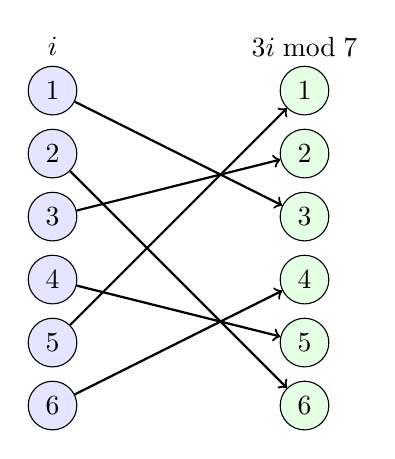
\begin{tikzpicture}[scale=0.8]
    \foreach \i in {1,...,6} {
        \node[circle,draw,fill=blue!10] (L\i) at (0, 7-\i) {$\i$};
        \node[circle,draw,fill=green!10] (R\i) at (4, 7-\i) {$\i$};
    }
    \draw[->,thick] (L1) -- (R3);
    \draw[->,thick] (L2) -- (R6);
    \draw[->,thick] (L3) -- (R2);
    \draw[->,thick] (L4) -- (R5);
    \draw[->,thick] (L5) -- (R1);
    \draw[->,thick] (L6) -- (R4);
    \node at (0, 6.7) {$i$};
    \node at (4, 6.7) {$3i \bmod 7$};
\end{tikzpicture}
\end{center}

让我们将这个例子稍作展开。从图中我们可以得出：
\[
\{1, 2, \dots, 6\} = \{3 \cdot 1 \bmod 7,\; 3 \cdot 2 \bmod 7,\; \dots,\; 3 \cdot 6 \bmod 7\}.
\]
将两种表示中的所有数字分别相乘，得到 $6! \equiv 3^6 \cdot 6! \pmod 7$；两边同时除以 $6!$，即得 $3^6 \equiv 1 \pmod 7$，这恰好就是 $a = 3, p = 7$ 时我们想要的结果。

现在我们将这一论证推广到一般的 $a$ 和素数 $p$，其中 $S = \{1, 2, \dots, p-1\}$。我们将证明当 $S$ 的元素在模 $p$ 下乘以 $a$ 时，得到的数字全部互不相同且非零。又因为它们都落在区间 $[1, p-1]$ 内，它们必然只是 $S$ 的一个置换。

数字 $a \cdot i \bmod p$ 互不相同，因为如果 $a \cdot i \equiv a \cdot j \pmod p$，两边除以 $a$ 便得到 $i \equiv j \pmod p$。它们是非零的，因为 $a \cdot i \equiv 0 \pmod p$ 同样意味着 $i \equiv 0$。（我们之所以能够除以 $a$，是因为根据假设 $a$ 非零且与素数 $p$ 互质。）

现在我们有两种方式表示集合 $S$：
\[
S = \{1, 2, \dots, p-1\} = \{a \cdot 1 \bmod p,\; a \cdot 2 \bmod p,\; \dots,\; a \cdot (p-1) \bmod p\}.
\]
将两种表示中的元素分别连乘，得到：
\[
(p-1)! \equiv a^{p-1} \cdot (p-1)! \pmod p.
\]
由于 $p$ 是素数，$(p-1)!$ 与 $p$ 互质，两边同时除以 $(p-1)!$ 即证明了定理。
\end{proof}

\begin{sidebarbox}{你的社会安全号码是素数吗？ (Is your social security number a prime?)}
数字 7, 17, 19, 71 和 79 都是素数，但 717-19-7179 呢？判断一个相当大的数字是否为素数似乎非常枯燥乏味，因为有太多的候选因子需要尝试。不过，有一些聪明的技巧可以加速这一过程。例如，在排除了 2 之后，你可以略去所有偶数候选因子；你实际上可以略去除了素数本身之外的所有候选因子。

事实上，稍加思考便可确信：只要排除了所有直到 $\sqrt{N}$ 的候选因子，就可以宣布 $N$ 是素数，因为如果 $N$ 确实可以分解为 $N = K \cdot L$，那么两个因子不可能同时大于 $\sqrt{N}$。

我们似乎在取得进展！也许通过省略越来越多的候选因子，就能发现真正高效的素性测试。

不幸的是，沿着这条道路走下去\textbf{根本无法得到快速的素性测试}。原因在于我们一直在试图通过“分解质因数”来判断一个数是否为素数。而因数分解是一个极其困难的问题！现代密码学以及本章后续内容都建立在以下重大核心思想之上：\textbf{因数分解极难，而素性测试极易}。我们无法轻易分解大数，但我们可以轻松测试巨大的数字是否为素数！（按理说，如果一个数是合数，测试会在无需找出其具体因数的情况下直接将其侦测出来。）
\end{sidebarbox}

费马小定理启发了一种无需因数分解的素数测试思路：
\begin{center}
\begin{tikzpicture}[node distance=2.5cm, auto]
    \node [draw, rectangle, rounded corners] (input) {挑选某个 $a < N$};
    \node [draw, diamond, aspect=2, below of=input, node distance=1.8cm] (test) {$a^{N-1} \equiv 1 \pmod N$ ?};
    \node [draw, rectangle, rounded corners, fill=green!20, below left of=test, node distance=2.5cm] (prime) {“素数” (Pass)};
    \node [draw, rectangle, rounded corners, fill=red!20, below right of=test, node distance=2.5cm] (comp) {“合数” (Fail)};
    
    \draw[->,thick] (input) -- (test);
    \draw[->,thick] (test) -| node[above,pos=0.3] {通过 (Yes)} (prime);
    \draw[->,thick] (test) -| node[above,pos=0.3] {未通过 (No)} (comp);
\end{tikzpicture}
\end{center}

问题在于：费马小定理并不是充要条件；它并没有断言当 $N$ 不是素数时会发生什么，因此在这些情况下上述流程图存疑。事实上，合数 $N$ 在特定基数 $a$ 的选择下也有可能通过费马测试（即 $a^{N-1} \equiv 1 \bmod N$）。例如 $341 = 11 \times 31$ 不是素数，但却有 $2^{340} \equiv 1 \pmod{341}$。尽管如此，我们依然希望对于合数 $N$ 而言，绝大多数 $a$ 的取值都会使测试失败。在即将精确阐述的意义下，这确实是成立的，这也启发了图 \ref{fig:primality_basic} 中的算法：与其预先固定一个任意的 $a$ 值，不如从 $\{1, \dots, N-1\}$ 中\textbf{随机}挑选它。

\begin{figure}[htbp]
\centering
\begin{tcolorbox}[colback=white,colframe=gray!50!black,title={\textbf{图 1.7}\quad 素性测试算法 (基础版)}]
\begin{algorithmic}[1]
\Function{primality}{$N$}
    \State \textbf{Input:} 正整数 $N$
    \State \textbf{Output:} yes/no
    \State 在区间 $[1, N-1]$ 中随机选取一个正整数 $a$
    \If{$a^{N-1} \equiv 1 \pmod N$}
        \State \Return yes
    \Else
        \State \Return no
    \EndIf
\EndFunction
\end{algorithmic}
\end{tcolorbox}
\label{fig:primality_basic}
\end{figure}

在分析该算法的行为时，我们首先需要排除一个极少数的不良特例。事实证明，存在一类极其罕见的合数 $N$（称为\textbf{卡迈克尔数}，Carmichael numbers），它们对所有与 $N$ 互质的 $a$ 都能通过费马测试。在这些数上我们的简单算法会失效；但它们极其病态罕见，我们稍后将讨论如何对付它们（第 28 页边栏），因此暂且忽略这类数。

在一个没有卡迈克尔数的世界中，我们的算法表现极其优秀。任何素数 $N$ 自然都会通过费马测试并产生正确答案。另一方面，任何非卡迈克尔合数 $N$ 必定会对某个 $a$ 无法通过费马测试；正如我们即将证明的，这直接意味着 $N$ 将对\textbf{至少一半}可能的 $a$ 值测试失败！

\begin{lemma}
若对于某个与 $N$ 互质的 $a$ 有 $a^{N-1} \not\equiv 1 \pmod N$，则对于至少一半的 $a < N$，该同余式不成立。
\end{lemma}

\begin{proof}
固定一个使得 $a^{N-1} \not\equiv 1 \pmod N$ 的 $a$ 值。关键在于注意到：每一个关于 $N$ 能通过费马测试的元素 $b < N$（即满足 $b^{N-1} \equiv 1 \pmod N$），都存在一个“孪生伴侣” $a \cdot b \bmod N$ 无法通过测试：
\[
(a \cdot b)^{N-1} \equiv a^{N-1} \cdot b^{N-1} \equiv a^{N-1} \cdot 1 \equiv a^{N-1} \not\equiv 1 \pmod N.
\]
此外，对于固定的 $a$ 和不同的 $b$，所有这些元素 $a \cdot b \bmod N$ 都是两两互不相同的，原因与费马测试证明中 $a \cdot i \not\equiv a \cdot j$ 完全相同：两边同除以 $a$ 即可。

\begin{center}
\begin{tikzpicture}[scale=0.9]
    \draw[thick, fill=green!10] (0,0) rectangle (3,3);
    \draw[thick, fill=red!10] (4,0) rectangle (7,3);
    \node at (1.5, 3.3) {\textbf{通过测试 (Pass)}};
    \node at (5.5, 3.3) {\textbf{未通过测试 (Fail)}};
    \node[circle,fill=black,inner sep=1.5pt,label=left:{$b$}] (b) at (1.5,1.5) {};
    \node[circle,fill=black,inner sep=1.5pt,label=right:{$a \cdot b$}] (ab) at (5.5,1.5) {};
    \draw[->,thick,blue] (b) to[bend left=20] node[above] {$b \mapsto a \cdot b$} (ab);
    \node at (3.5,-0.5) {集合 $\{1, 2, \dots, N-1\}$ 的映射划分};
\end{tikzpicture}
\end{center}

单射函数 $b \mapsto a \cdot b \bmod N$ 表明，导致测试失败的元素数量至少与通过测试的元素数量一样多。
\end{proof}

忽略卡迈克尔数后，我们现在可以断言：
\begin{itemize}
    \item 若 $N$ 是素数，则对所有 $a < N$ 均有 $a^{N-1} \equiv 1 \pmod N$。
    \item 若 $N$ 是合数，则至多对一半的 $a < N$ 满足 $a^{N-1} \equiv 1 \pmod N$。
\end{itemize}

因此图 \ref{fig:primality_basic} 算法具有如下概率行为：
\begin{align*}
\Pr(\text{算法 \ref{fig:primality_basic} 在 } N \text{ 为素数时返回 yes}) &= 1, \\
\Pr(\text{算法 \ref{fig:primality_basic} 在 } N \text{ 为合数时返回 yes}) &\le \frac{1}{2}.
\end{align*}

\begin{sidebarbox}{嘿，那是群论！ (Hey, that was group theory!)}
对于任意整数 $N$，模 $N$ 下所有与 $N$ 互质的数的集合构成了数学家所称的\textbf{群 (group)}：
\begin{itemize}
    \item 该集合上定义了乘法运算。
    \item 该集合包含一个单位元（即 1：任何数乘以 1 保持不变）。
    \item 所有元素都拥有良定义的逆元。
\end{itemize}
这个特殊的群被称为模 $N$ 的\textbf{乘法群}，通常记作 $\mathbb{Z}_N^*$。

群论是数学中一个高度成熟的分支。其核心概念之一是群可以包含\textbf{子群 (subgroup)}——即本身也构成群的子集。关于子群的一个重要基本事实是：\textbf{子群的大小必须整除整个群的大小}（拉格朗日定理）。

现在考虑集合 $B = \{b \in \mathbb{Z}_N^* : b^{N-1} \equiv 1 \pmod N\}$。不难看出它是 $\mathbb{Z}_N^*$ 的一个子群（只需验证 $B$ 在乘法和逆元下封闭）。因此 $B$ 的大小必须整除 $\mathbb{Z}_N^*$ 的大小。这意味着如果 $B$ 不包含 $\mathbb{Z}_N^*$ 的全部元素，它所能拥有的下一个最大可能规模就是 $|\mathbb{Z}_N^*| / 2$。
\end{sidebarbox}

我们可以通过多次重复该过程，随机选取若干个 $a$ 值并全部进行测试，从而大幅降低这种单向错误率（图 \ref{fig:primality_robust}）。

\begin{figure}[htbp]
\centering
\begin{tcolorbox}[colback=white,colframe=gray!50!black,title={\textbf{图 1.8}\quad 具有极低错误概率的素性测试算法}]
\begin{algorithmic}[1]
\Function{primality2}{$N, k$}
    \State \textbf{Input:} 正整数 $N$，重复次数 $k$
    \State \textbf{Output:} yes/no
    \State 在区间 $[1, N-1]$ 中随机独立选取 $k$ 个正整数 $a_1, a_2, \dots, a_k$
    \If{对所有 $i = 1, 2, \dots, k$ 均有 $a_i^{N-1} \equiv 1 \pmod N$}
        \State \Return yes
    \Else
        \State \Return no
    \EndIf
\EndFunction
\end{algorithmic}
\end{tcolorbox}
\label{fig:primality_robust}
\end{figure}

此时的错误概率上限为：
\[
\Pr(\text{算法 \ref{fig:primality_robust} 在 } N \text{ 为合数时返回 yes}) \le \frac{1}{2^k}.
\]
这种错误概率以指数级的速度衰减，通过选择足够大的 $k$ 可以使其降至任意低。例如测试 $k = 100$ 个 $a$ 值，失误概率至多为 $2^{-100}$，这是一个微不足道的极小概率：甚至远低于在计算过程中宇宙射线随机击中并破坏计算机芯片的概率！

\begin{sidebarbox}{卡迈克尔数 (Carmichael numbers)}
最小的卡迈克尔数是 561。它不是素数：$561 = 3 \times 11 \times 17$；然而它欺骗了费马测试，因为对于所有与 561 互质的 $a$，都有 $a^{560} \equiv 1 \pmod{561}$。长期以来人们曾以为这类数可能只有有限多个；现在我们知道它们有无穷多个，但极其罕见。

利用由 Rabin 和 Miller 提出的更精细的素性测试，可以完美避开卡迈克尔数。将 $N - 1$ 写成 $2^t u$ 的形式（其中 $u$ 为奇数）。如同之前一样，我们随机选取基数 $a$，并检查 $a^{N-1} \bmod N$ 的值。通过首先计算 $a^u \bmod N$，然后连续进行平方，得到序列：
\[
a^u \bmod N,\; a^{2u} \bmod N,\; \dots,\; a^{2^t u} \equiv a^{N-1} \bmod N.
\]
若 $a^{N-1} \not\equiv 1 \pmod N$，由费马小定理可知 $N$ 必为合数，测试结束。
但若 $a^{N-1} \equiv 1 \pmod N$，我们进行后续检查：在上述序列中，我们在某个位置第一次碰到了 1。如果这发生在第一个位置之后（即 $a^u \bmod N \ne 1$），且列表中紧随其前的值不等于 $-1 \bmod N$，我们就判定 $N$ 为合数。

在后一种情况下，我们实际上找到了 1 模 $N$ 的一个\textbf{非平凡平方根}：一个模 $N$ 下不等于 $\pm 1$ 但平方后却模 $N$ 同余于 1 的数。这样的数唯有在 $N$ 为合数时才会存在（参见习题 1.40）。事实证明，如果将这种平方根检验与先前的费马测试结合起来，那么在 1 到 $N-1$ 之间至少有四分之三的 $a$ 值能够揭穿合数 $N$，即便它是卡迈克尔数也不例外。
\end{sidebarbox}

\subsection{生成随机素数 (Generating random primes)}
我们现在即将凑齐密码学应用所需的全部工具。最后一块拼图是快速挑选长达数百位的随机素数的算法。这项任务之所以相当容易，是因为\textbf{素数极为丰富}——一个随机的 $n$ 位数字大约有 $1/n$ 的概率是素数（更精确地说是约 $1/(\ln 2^n) \approx 1.44/n$）。例如，大约每 20 个社会安全号码中就有 1 个是素数！

\begin{theorem}[\textbf{拉格朗日素数定理 (Lagrange's prime number theorem)}]
设 $\pi(x)$ 为不超过 $x$ 的素数个数，则 $\pi(x) \approx x / \ln x$，更准确地说：
\[
\lim_{x \to \infty} \frac{\pi(x)}{x / \ln x} = 1.
\]
\end{theorem}

这种丰富性使得生成一个随机 $n$ 位素数变得极为简单：
\begin{itemize}
    \item 随机选取一个 $n$ 位的数字 $N$。
    \item 对 $N$ 运行素性测试。
    \item 若通过测试则输出 $N$；否则重复上述过程。
\end{itemize}

该算法有多快？如果随机选取的 $N$ 确实是素数（发生概率至少为 $1/n$），它必定能通过测试。因此在每次迭代中，该过程至少有 $1/n$ 的概率停机。因此平均而言，它将在 $O(n)$ 轮内停机（参见习题 1.34）。

接下来，具体应该使用哪种素性测试？在此应用中，由于待测试的数字是随机挑选而非敌手刻意构造的，通常只需使用以 $a = 2$ 为底的费马测试（或者为了万无一失，使用 $a = 2, 3, 5$），因为对于随机数字，费马测试的失误概率远小于我们先前证明的最坏情况 $1/2$ 上界。通过这种测试的数字常被戏称为“工业级素数”（industrial grade primes）。由此得到的算法非常快，在个人电脑上只需几分之一秒就能生成长达数百位的素数。

\begin{sidebarbox}{随机化算法：虚拟章节 (Randomized algorithms: a virtual chapter)}
令人惊讶——甚至近乎悖论——的是，我们拥有的一些最快速、最精妙的算法竟然依赖于偶然性：在特定步骤中，它们根据随机抛硬币的结果来决定下一步行动。这些\textbf{随机化算法}通常极其简洁优雅，并且允许其输出以极小的概率出错。这种对失败概率的上界对\textbf{每一个}输入均成立；它仅仅取决于算法自身所做的随机选择，并且可以轻易压缩至任意小的程度。

本书没有为该主题设立专门章节，而是将随机化算法分散穿插在它们最自然出现的章节和章节中。此外，理解这些内容不需要高深的专门概率知识。你只需要熟悉概率的基本概念、期望值、抛硬币直到出现正面所需的期望次数，以及所谓的“期望线性性”即可。

以下是本书中主要随机化算法的索引：
\begin{itemize}
    \item 随机化算法最早也是最引人注目的例子之一，就是图 \ref{fig:primality_robust} 中的概率素性测试。尽管最近发现了确定性素性测试（AKS 算法），但随机测试要快得多，因此仍然是首选算法。
    \item 在本章稍后的第 1.5 节（第 35 页），我们将讨论哈希（Hashing），这是一种通用的随机化数据结构，支持插入、删除和查找。在实践中，它比二叉搜索树等确定性方案能带来更快的数据访问。
    \item 随机化算法主要分为两类：\textbf{蒙特卡洛算法 (Monte Carlo)} 总是运行很快，但其输出有小概率出错（素性测试就是典型代表）；而 \textbf{拉斯维加斯算法 (Las Vegas)} 总是输出正确答案，但以高概率保证较短的运行时间（例如第 2 章第 50 页和第 53 页介绍的快速排序与中位数查找）。
    \item 目前已知求解最小割问题的最快算法是随机化蒙特卡洛算法（第 139 页边栏）。
    \item 随机化在启发式算法中也扮演着重要角色（第 9.3 节）。
    \item 最后，用于大数分解的量子算法（第 10.7 节）非常类似于随机化算法，其输出以高概率正确——不同之处在于它的随机性不是来自抛硬币，而是来自量子力学中的叠加原理。
\end{itemize}
虚拟习题：1.29, 1.34, 1.46, 2.24, 2.33, 5.35, 9.8, 10.8。
\end{sidebarbox}

剩下的重要问题是：算法输出的结果真正是素数的概率有多大？为了回答这一问题，我们必须理解费马测试的辨别力有多强。举一个具体的例子，假设我们对所有 $N \le 25 \times 10^9$ 的数字执行以 $a = 2$ 为底的测试。在这一范围内，大约有 $10^9$ 个素数，而通过测试的合数仅有约 20,000 个。因此，错误输出合数的概率大约为 $20,000 / 10^9 = 2 \times 10^{-5}$。随着所涉及数字长度的增加（达到我们应用中所期望的数百位数字），这种出错概率会极速衰减。

\section{密码学 (Cryptography)}

我们的下一个主题——Rivest-Shamir-Adleman (RSA) 密码体制，综合运用了本章介绍的所有思想！它通过巧妙利用某些数论任务的多项式时间可计算性（模幂运算、最大公约数、素性测试）与另一些任务的难解性（质因数分解）之间的巨大鸿沟，获得了极其坚固的安全保证。

密码学的典型场景可以通过三个人物构成的角色设定来描述：Alice 和 Bob 希望进行保密通信，而 Eve 是一名窃听者，会竭尽全力探听他们的谈话内容。具体而言，假设 Alice 想给她的朋友 Bob 发送一条用二进制表示的消息 $x$。她将其编码为 $e(x)$ 发送出去，随后 Bob 应用他的解密函数 $d(\cdot)$ 进行解码：$d(e(x)) = x$。这里 $e(\cdot)$ 和 $d(\cdot)$ 是对消息的合适变换映射。

\begin{figure}[htbp]
\centering
\begin{tikzpicture}[>=latex, auto, node distance=2.2cm]
    \node[draw, rectangle, rounded corners, fill=blue!10] (alice) {Alice (发送方)};
    \node[draw, rectangle, right of=alice, node distance=3.2cm] (enc) {加密器 $e(\cdot)$};
    \node[draw, rectangle, right of=enc, node distance=3.5cm] (dec) {解密器 $d(\cdot)$};
    \node[draw, rectangle, rounded corners, fill=blue!10, right of=dec, node distance=3.2cm] (bob) {Bob (接收方)};
    \node[draw, rectangle, rounded corners, fill=red!10, above of=enc, node distance=1.8cm, xshift=1.75cm] (eve) {Eve (窃听者)};

    \draw[->, thick] (alice) -- node[above] {$x$} (enc);
    \draw[->, thick] (enc) -- node[above] {$e(x)$} (dec);
    \draw[->, thick] (dec) -- node[above] {$x = d(e(x))$} (bob);
    \draw[->, thick, dashed, red] (1.75,0) -- (eve);
\end{tikzpicture}
\caption{保密通信模型}
\label{fig:crypto_model}
\end{figure}

Alice 和 Bob 担心窃听者 Eve 会截获 $e(x)$（例如她可能是网络上的嗅探器）。但在理想情况下，加密函数 $e(\cdot)$ 的设计使得在不知道 $d(\cdot)$ 的情况下，Eve 无法从获取的信息中得到任何好处。换句话说，获知 $e(x)$ 几乎或完全无法让她推断出 $x$ 可能是什么。

几个世纪以来，密码学都基于我们现在所称的\textbf{私钥体制}（对称密钥体制）。在这样的方案中，Alice 和 Bob 预先秘密会面并共同商定一本密码本，用它来加密未来彼此之间的一切通信。此时 Eve 唯一的希望就是收集一些密文消息，并尝试利用它们至少部分破解出密码本。

像 RSA 这样的\textbf{公钥体制}（非对称密钥体制）则要精妙高超得多：它们允许 Alice 在从未与 Bob 见过面的情况下直接向 Bob 发送保密消息。Bob 的加密函数 $e(\cdot)$ 是完全公开的，Alice 可以使用该函数加密她的消息，从而在数字层面上将其“上锁”。唯有 Bob 拥有快速解开这把数字锁的钥匙——解密函数 $d(\cdot)$。关键在于，Alice 和 Bob 各自只需执行简单的计算来完成上锁和解锁——这些操作任何掌上计算设备都能轻松胜任。相比之下，要在没有密钥的情况下强行解锁，Eve 必须执行诸如大整数质因数分解之类的操作，这需要的计算能力甚至超过全世界最强大的计算机总和。这一令人信服的保证使得安全的网络电子商务（例如通过互联网向公司发送信用卡号）成为现实。

\subsection{私钥体制：一次一密与 AES (Private-key schemes: one-time pad and AES)}
如果 Alice 想要向 Bob 发送一条重要的机密消息，明智的做法是用一个加密函数将其打乱混淆：
\[
e : \{\text{明文消息}\} \to \{\text{密文消息}\}.
\]
当然，该函数必须是可逆的——以便能够进行解码——因此它是一个双射（双向一一映射）。其反函数即为解密函数 $d(\cdot)$。

在\textbf{一次一密 (one-time pad)} 中，Alice 和 Bob 预先会面并秘密选择一个与 Alice 后续将要发送的重要消息 $x$ 具有相同长度（例如 $n$ 比特）的随机二进制字符串 $r$。Alice 的加密函数是逐比特异或（exclusive-or）：$e_r(x) = x \oplus r$：密文中的每个位置都是 $x$ 和 $r$ 对应位置的异或。例如，若 $r = 01110010$，则消息 $11110000$ 将被混淆如下：
\[
e_r(11110000) = 11110000 \oplus 01110010 = 10000010.
\]
该函数 $e_r$ 是从 $n$ 比特字符串到 $n$ 比特字符串的双射，因为它本身就是自己的反函数：
\[
e_r(e_r(x)) = (x \oplus r) \oplus r = x \oplus (r \oplus r) = x \oplus \bm{0} = x,
\]
其中 $\bm{0}$ 是全零字符串。因此 Bob 只需将相同的加密函数再次应用一次即可解码：$d_r(y) = y \oplus r$。

Alice 和 Bob 应该如何挑选 $r$ 才能确保该方案绝对安全？很简单：他们应该\textbf{完全随机}地挑选 $r$（对每一位独立抛硬币），使得生成的字符串等概率地取遍 $\{0, 1\}^n$ 中的任何元素。这将确保即使 Eve 截获了密文 $y = e_r(x)$，她也无法获得关于 $x$ 的任何信息。例如假设 Eve 获知 $y = 10$；她能推断出什么？她不知道 $r$，而 $r$ 所有可能的取值分别对应于不同的原始消息 $x$：
\begin{center}
\begin{tikzpicture}[scale=0.8]
    \node (x00) at (0, 3) {$00$};
    \node (x01) at (0, 2) {$01$};
    \node (x10) at (0, 1) {$10$};
    \node (x11) at (0, 0) {$11$};
    \node at (0, 3.7) {\textbf{明文} $x$};

    \node (y) at (5, 1.5) {$y = 10$};
    \node at (5, 3.7) {\textbf{密文} $y$};

    \draw[->,thick] (x00) -- node[above,sloped,font=\scriptsize] {$r=10$} (y);
    \draw[->,thick] (x01) -- node[above,sloped,font=\scriptsize] {$r=11$} (y);
    \draw[->,thick] (x10) -- node[above,sloped,font=\scriptsize] {$r=00$} (y);
    \draw[->,thick] (x11) -- node[above,sloped,font=\scriptsize] {$r=01$} (y);
\end{tikzpicture}
\end{center}
因此根据 Eve 所掌握的信息，$x$ 的所有可能取值都是完全等可能的！

一次一密的缺点在于它在单次使用后必须彻底废弃，这也是其名称的由来。使用相同的密钥串对第二条消息进行加密将不再安全，因为如果 Eve 获得了两条消息 $x$ 和 $z$ 的密文 $x \oplus r$ 与 $z \oplus r$，她就可以将它们进行异或运算得到 $(x \oplus r) \oplus (z \oplus r) = x \oplus z$，这可能暴露出极其重要的信息——例如：(1) 它揭示了两条消息的开头或结尾是否相同；(2) 如果某条消息包含很长一段连续的零（若消息是图像则极可能如此），那么另一条消息的对应部分将被直接暴露。因此，Alice 和 Bob 共享的随机字符串长度必须等于他们未来需要交换的所有消息长度的总和。

一次一密是一个理论性质完全透明的教学玩具式密码方案。位于光谱另一端的是\textbf{高级加密标准 (AES)}，这是美国国家标准与技术研究院（NIST）于 2001 年批准的广泛应用的密码协议。AES 同样是私钥体制：Alice 和 Bob 必须商定一个共享的随机字符串 $r$。但这次该密钥字符串具有较小的固定大小（精确地说是 128 比特，也有 192 或 256 比特的变体），并定义了一个从 128 位串到 128 位串的双射 $e_r$。关键区别在于：该函数可以被\textbf{反复使用}，例如可以通过将长消息切分成 128 比特的块，并对每个块分别应用 $e_r$ 来完成加密。

AES 的安全性尚未在理论上得到严格证明，但毫无疑问，目前公众除了暴力穷举共享密钥串 $r$ 的所有可能之外，尚不知道如何有效破解它。

\subsection{RSA 体制 (RSA)}
与前两种协议不同，RSA 方案是\textbf{公钥密码学}的典范：任何人都可以使用公开可用的信息（类似于公开的通信地址或电话号码）向其他人发送保密消息。每个人都拥有一把全世界皆知的\textbf{公钥}，以及一把仅有自己知晓的\textbf{私钥（秘钥）}。当 Alice 想给 Bob 发送消息 $x$ 时，她使用 Bob 的公钥对其加密。Bob 使用自己的私钥进行解密，从而恢复出 $x$。Eve 可以随意查看发给 Bob 的任意多条密文消息，但在一些简单的假设下，她将完全无法解码它们。

RSA 方案深度依赖数论。将 Alice 发送给 Bob 的消息视为模 $N$ 的数字；大于 $N$ 的长消息可以拆分为较小的块。加密函数将是集合 $\{0, 1, \dots, N-1\}$ 上的双射，而解密函数则是它的逆映射。什么样的 $N$ 才是合适的？应该采用什么样的双射？

\begin{property}
任意选取两个质数 $p$ 和 $q$，令 $N = pq$。对于任意与 $(p-1)(q-1)$ 互质的整数 $e$：
\begin{enumerate}
    \item 映射 $x \mapsto x^e \bmod N$ 是集合 $\{0, 1, \dots, N-1\}$ 上的双射。
    \item 此外，其逆映射极易实现：令 $d$ 为 $e$ 模 $(p-1)(q-1)$ 的乘法逆元。则对所有 $x \in \{0, \dots, N-1\}$，均有：
    \[
    (x^e)^d \equiv x \pmod N.
    \]
\end{enumerate}
\end{property}

第一条性质告诉我们，映射 $x \mapsto x^e \bmod N$ 是一种合理的编码方式；信息完全不会丢失。因此，如果 Bob 将 $(N, e)$ 作为公钥发布，任何人都可以用它向他发送加密消息。第二条性质则告诉我们如何进行解密。Bob 应当保留 $d$ 作为私钥，收到密文后，只需在模 $N$ 下对密文求 $d$ 次方即可完成解码。

\begin{example}
令 $N = 55 = 5 \times 11$。选取加密指数 $e = 3$，它满足 $\gcd(e, (p-1)(q-1)) = \gcd(3, 40) = 1$。解密指数为 $d = 3^{-1} \bmod 40 = 27$。对于任意消息 $x \bmod 55$，$x$ 的密文为 $y = x^3 \bmod 55$，而对 $y$ 解密得到 $x = y^{27} \bmod 55$。例如若明文 $x = 13$，则密文 $y = 13^3 = 2197 \equiv 52 \pmod{55}$；解密则为 $52^{27} \equiv 13 \pmod{55}$。
\end{example}

让我们证明上述断言，然后剖析该方案的安全性。

\begin{proof}
如果映射 $x \mapsto x^e \bmod N$ 是可逆的，则它必定是双射；因此命题 2 蕴含命题 1。为了证明命题 2，我们首先注意到由于 $e$ 与 $(p-1)(q-1)$ 互质，故 $e$ 模 $(p-1)(q-1)$ 的逆元必然存在。为了证明 $(x^e)^d \equiv x \pmod N$，我们审视其指数：由于 $ed \equiv 1 \pmod{(p-1)(q-1)}$，我们可以将 $ed$ 写成 $1 + k(p-1)(q-1)$ 的形式（其中 $k$ 为某个整数）。现在我们需要证明差值：
\[
x^{ed} - x = x^{1 + k(p-1)(q-1)} - x
\]
永远在模 $N$ 下为 0。该表达式的第二种形式非常便于利用费马小定理进行化简。它能被 $p$ 整除（因为若 $x$ 不是 $p$ 的倍数，则 $x^{p-1} \equiv 1 \pmod p$，故 $x(x^{p-1})^{k(q-1)} - x \equiv x \cdot 1 - x \equiv 0 \pmod p$；若 $x$ 是 $p$ 的倍数，显然同余于 0）；同理它也能被 $q$ 整除。由于 $p$ 和 $q$ 是互异的素数，该表达式必能被它们的乘积 $N = pq$ 整除。因此：
\[
x^{ed} - x = x^{1 + k(p-1)(q-1)} - x \equiv 0 \pmod N,
\]
这正是我们所需要的结论。
\end{proof}

\begin{figure}[htbp]
\centering
\begin{tcolorbox}[colback=white,colframe=gray!50!black,title={\textbf{图 1.9}\quad RSA 密码体制流程}]
\textbf{Bob 生成他的公钥与私钥：}
\begin{itemize}
    \item 首先随机挑选两个巨大的（$n$ 位）素数 $p$ 和 $q$。
    \item 他的\textbf{公钥}为 $(N, e)$，其中 $N = pq$，$e$ 是一个与 $(p-1)(q-1)$ 互质的 $2n$ 位整数。常见的选择是 $e = 3$（或 65537），因为这允许极快的加密。
    \item 他的\textbf{私钥}为 $d$，即 $e$ 模 $(p-1)(q-1)$ 的乘法逆元，使用扩展欧几里得算法计算得出。
\end{itemize}
\textbf{Alice 希望向 Bob 发送消息 $x$：}
\begin{itemize}
    \item 她查阅 Bob 的公钥 $(N, e)$，利用高效的模幂算法计算并发送 $y = (x^e \bmod N)$。
    \item Bob 收到后，通过计算 $y^d \bmod N$ 解码出原始消息。
\end{itemize}
\end{tcolorbox}
\label{fig:rsa_protocol}
\end{figure}

RSA 协议在图 \ref{fig:rsa_protocol} 中进行了总结。它无疑是极其便利的：它要求 Alice 和 Bob 执行的计算都是非常基础的初等运算。但是面对 Eve 时，它究竟有多安全？

RSA 的安全性建立在一个简单的计算假设之上：
\begin{center}
    \textbf{给定 $N, e$ 以及 $y = x^e \bmod N$，在计算上确定 $x$ 是不可行的。}
\end{center}
这个假设是高度可信的。Eve 可能会如何尝试猜测 $x$？她可以尝试 $x$ 的所有可能取值，每次检查是否满足 $x^e \equiv y \pmod N$，但这需要耗费指数级的时间。或者她可以尝试对 $N$ 进行质因数分解以找回 $p$ 和 $q$，进而通过对 $e$ 求模 $(p-1)(q-1)$ 的逆元来计算出 $d$；但我们普遍相信因数分解是极其困难的。计算难解性通常令人沮丧；而 RSA 的卓越洞见正在于\textbf{化难解性为巨大优势}。

\section{全域哈希 (Universal hashing)}

我们以数论在哈希函数设计中的应用来结束本章。哈希（散列）是一种极其有用的数据组织方式，用于在表中存储数据项，以支持高效的插入、删除和查找操作。

假设我们需要维护一个不断变化的、包含约 250 个 IP（互联网协议）地址的列表，例如某 Web 服务的当前活跃客户地址。（回忆一下，IP 地址由 32 个比特组成，编码了计算机在互联网上的位置，通常表示为四个 8 位的字段，例如 128.32.168.80）。如果我们用以 IP 地址为索引的巨大数组来维护这些记录，固然可以获得极快的查找时间。但这对内存是极大的浪费：该数组将拥有 $2^{32} \approx 4 \times 10^9$ 个表项，其中绝大部分都处于空闲状态。或者，我们也可以使用仅包含这 250 条记录的链表。但此时访问记录将会非常缓慢，所需时间与客户总数 250 呈正比。是否存在兼得两者之长的方法——使用的内存量与客户数量成正比，同时还能实现快速查找？这正是哈希大显身手之处。

\subsection{哈希表 (Hash tables)}
以下是哈希的高层视角。我们将为 $2^{32}$ 个可能的 IP 地址中的每一个赋予一个简短的“昵称”。你可以把这个短名称看作仅仅是 1 到 250 之间的一个数字（稍后我们会对该范围进行微调）。因此，必然会有许多 IP 地址具有相同的昵称；然而，我们希望我们特定客户的 250 个 IP 地址大部分都被分配到互不相同的名字，我们将它们存储在一个大小约为 250、以这些名字为索引的数组中。如果同一个名字关联了多条记录该怎么办？很简单：数组的每个表项都指向一个包含所有同名记录的链表（拉链法）。因此总存储量与客户数量 250 成正比，而与可能的 IP 地址总数无关。此外，只要分配到同一个名字的客户 IP 地址数量不多，查找就会非常快，因为我们需要扫描的链表平均长度极小。

\begin{figure}[htbp]
\centering
\begin{tikzpicture}[scale=0.85]
    \draw[thick, fill=blue!5] (0,0) ellipse (1.8cm and 2.5cm);
    \node at (0, 2) {\textbf{全部 $2^{32}$ 个 IP 地址空间}};
    \node[circle,fill=black,inner sep=1.2pt,label=left:$x$] (x) at (-0.5,0.8) {};
    \node[circle,fill=black,inner sep=1.2pt,label=left:$y$] (y) at (0.2,0.1) {};
    \node[circle,fill=black,inner sep=1.2pt,label=left:$z$] (z) at (-0.3,-1.2) {};
    \node at (0, -2) {\footnotesize 包含250个活跃IP};

    \draw[thick] (6,-2.5) rectangle (8,2.5);
    \foreach \i in {-2,-1.5,...,2} {
        \draw (6,\i) -- (8,\i);
    }
    \node at (7, 2.8) {\textbf{大小 $\approx 250$ 的哈希表}};

    \draw[->,thick,blue] (x) to[bend left=20] node[above] {$h(x)$} (6, 1.25);
    \draw[->,thick,blue] (y) to[bend left=10] node[above] {$h(y)$} (6, 0.25);
    \draw[->,thick,blue] (z) to[bend right=20] node[below] {$h(z)$} (6, -1.75);

    \draw[fill=gray!20] (8.5, 1.1) rectangle (9.5, 1.4);
    \node[font=\scriptsize] at (9, 1.25) {记录 $x$};
    \draw[->] (7.5, 1.25) -- (8.5, 1.25);
\end{tikzpicture}
\caption{哈希表与映射示意图}
\label{fig:hash_table}
\end{figure}

但是我们如何为每个 IP 地址分配一个短名称？这就是\textbf{哈希函数}的职责：在我们的例子中，哈希函数 $h$ 将 IP 地址映射到长度约为 250 的表中的位置。IP 地址 $x$ 分配到的名字为 $h(x)$，而 $x$ 的记录就存储在表的第 $h(x)$ 个槽位中。如前所述，表的每个槽位实际上是一个“桶”（bucket）——一个包含映射到该位置的所有当前 IP 地址的链表。我们期望包含超过寥寥数个 IP 地址的桶极少出现。

\subsection{哈希函数族 (Families of hash functions)}
设计哈希函数非常棘手。哈希函数在某种意义上必须是“随机”的（以便将数据项均匀分散各处），但它又必须是一个确定性的数学函数，因而具有“一致性”（以便每次应用它时都能得到相同的结果）。

此外，数据项本身的统计分布可能会对我们不利。在我们的例子中，一种可能的哈希函数是将 IP 地址映射到其最后一段的 8 位数字：$h(128.32.168.80) = 80$。此时需要一个拥有 $n = 256$ 个桶的表。但这算是一个好的哈希函数吗？如果例如我们客户的 IP 地址末段往往是较小的数字（一位数或两位数），那么低编号的桶就会发生严重拥堵。使用 IP 地址的第一段同样容易招致灾难——例如，如果大多数客户都来自亚洲。

这两个函数本身并没有固有的错误。如果我们的 250 个 IP 地址是从全部 $N = 2^{32}$ 种可能中均匀随机选出的，那么这些函数的表现会相当不错。问题在于我们无法保证实际 IP 地址的分布是均匀的。

反过来讲，\textbf{没有任何单一的确定性哈希函数（无论设计得多么精巧复杂）能够在所有数据集上都表现良好}。由于哈希函数将 $2^{32}$ 个 IP 地址映射到仅 250 个名字，必然存在至少 $2^{32} / 250 \approx 2^{24} \approx 16,000,000$ 个被分配到相同名字的 IP 地址集合（在哈希术语中称为“冲突”，collision）。如果这些地址中有许多恰好出现在我们的客户集中，我们就会陷入巨大的麻烦。

显然，我们需要引入某种随机化。这里有一个绝妙的想法：\textbf{让我们从某个特定的函数族中随机挑选一个哈希函数}。然后我们将证明：无论我们实际关心的 250 个 IP 地址集合是怎样的，大多数哈希函数的选择都会在这些地址之间产生极少的冲突。

为此，我们需要定义一个可以从中进行随机选择的哈希函数族；而这正是数论大显身手之处。我们将桶的数量设定为不是 250，而是 $n = 257$——一个\textbf{素数}！我们把每个 IP 地址 $x$ 视为模 $n$ 的四元整数元组 $x = (x_1, x_2, x_3, x_4)$——回忆一下它原本就是 0 到 255 之间的四个整数，因此这样做完全没有任何问题。我们可以定义一个从 IP 地址到模 $n$ 数字的函数 $h$ 如下：在模 $n = 257$ 下任意固定四个数字，例如 87, 23, 125 和 4。现在将 IP 地址 $(x_1, \dots, x_4)$ 映射为：
\[
h(x_1, \dots, x_4) = (87x_1 + 23x_2 + 125x_3 + 4x_4) \bmod 257.
\]
事实上，模 $n$ 下的任意四个数字都定义了一个合法的哈希函数。

对于任意四个系数 $a_1, \dots, a_4 \in \{0, 1, \dots, n-1\}$，记 $\bm{a} = (a_1, a_2, a_3, a_4)$，并定义 $h_{\bm{a}}$ 为如下哈希函数：
\[
h_{\bm{a}}(x_1, \dots, x_4) = \sum_{i=1}^4 a_i \cdot x_i \bmod n.
\]

我们将证明，如果随机独立选取这些系数 $\bm{a}$，那么 $h_{\bm{a}}$ 在如下意义下极大概率是极佳的：

\begin{property}
考虑任意一对互异的 IP 地址 $x = (x_1, \dots, x_4)$ 和 $y = (y_1, \dots, y_4)$。若系数 $\bm{a} = (a_1, \dots, a_4)$ 是从 $\{0, 1, \dots, n-1\}$ 中独立均匀随机选取的，则：
\[
\Pr\{h_{\bm{a}}(x_1, \dots, x_4) = h_{\bm{a}}(y_1, \dots, y_4)\} = \frac{1}{n}.
\]
\end{property}

换句话说，$x$ 和 $y$ 在 $h_{\bm{a}}$ 下发生冲突的概率，与它们各自被随机独立分配昵称时的冲突概率完全相同。这一条件保证了任意数据项的期望查找时间极短。原因如下：如果我们要查找表中的 $x$，所需时间主要由其所在桶的大小（即被分配与 $x$ 相同名字的数据项数量）决定。但哈希表中总共只有 250 个数据项，任意单个数据项与 $x$ 分配到相同名字的概率为 $1/n = 1/257$。因此，随机选取的哈希函数 $h_{\bm{a}}$ 分配到与 $x$ 相同名字的数据项期望数量为 $250/257 \approx 1$，这意味着包含 $x$ 的桶的期望大小小于 2。\footnote{当随机选取哈希函数 $h_{\bm{a}}$ 时，令随机变量 $Y_i$（对 $i = 1, \dots, 250$）在第 $i$ 个数据项与 $x$ 获得相同名字时为 1，否则为 0。则 $Y_i$ 的期望值为 $1/n$。令 $Y = Y_1 + \cdots + Y_{250}$ 为与 $x$ 同名的数据项总数，由期望的线性性质，总期望值即为各期望值之和：$250/n = 250/257$。}

现在我们来证明上述性质。

\begin{proof}
由于 $x = (x_1, \dots, x_4)$ 和 $y = (y_1, \dots, y_4)$ 是互异的，这两个四元组必然在某个分量上不同；不妨设 $x_4 \ne y_4$。我们希望计算概率 $\Pr[h_{\bm{a}}(x) = h_{\bm{a}}(y)]$，即 $\sum_{i=1}^4 a_i x_i \equiv \sum_{i=1}^4 a_i y_i \pmod n$ 的概率。最后一个等式可以改写为：
\begin{equation}
\sum_{i=1}^3 a_i (x_i - y_i) \equiv a_4 (y_4 - x_4) \pmod n. \tag{1}
\end{equation}
假设我们通过随机抽取 $\bm{a} = (a_1, a_2, a_3, a_4)$ 来生成随机哈希函数 $h_{\bm{a}}$。我们首先独立抽取 $a_1, a_2, a_3$，然后停下来思考：最后抽取的数字 $a_4$ 使得方程 (1) 成立的概率是多少？

截至目前，方程 (1) 的左边计算为一个确定的数值，记为 $c$。由于 $n$ 是素数且 $x_4 \ne y_4$，根据模除法定理，$(y_4 - x_4)$ 模 $n$ 存在唯一的乘法逆元。因此为了使方程 (1) 成立，最后一个数字 $a_4$ 在其 $n$ 个可能取值中必须精确等于 $c \cdot (y_4 - x_4)^{-1} \bmod n$。这一事件发生的概率恰好是 $1/n$，证明完毕。
\end{proof}

让我们退后一步，总结我们刚刚取得的成果。由于我们无法控制输入的数据项集合，我们转而决定从一个哈希函数族 $\mathcal{H}$ 中均匀随机地选取哈希函数 $h$。在我们的例子中：
\[
\mathcal{H} = \{h_{\bm{a}} : \bm{a} \in \{0, \dots, n-1\}^4\}.
\]
要从该族中均匀随机抽取一个哈希函数，我们只需独立抽取四个模 $n$ 的数字 $a_1, \dots, a_4$。（顺便注意，我们先前考虑的两个简单哈希函数——取最后或第一个 8 位字段——恰好属于此类，它们分别对应于 $h_{(0,0,0,1)}$ 和 $h_{(1,0,0,0)}$）。我们坚持要求该函数族具备以下性质：
\begin{center}
    \textbf{对于任意两个互异的数据项 $x$ 和 $y$，$\mathcal{H}$ 中恰好有 $|\mathcal{H}|/n$ 的哈希函数将 $x$ 和 $y$ 映射到同一个桶，其中 $n$ 为桶的数量。}
\end{center}
具备这种性质的哈希函数族被称为\textbf{全域哈希族 (universal family of hash functions)}。换言之，如果哈希函数是从全域族中随机抽取的，则任意两个数据项发生冲突的概率恒为 $1/n$。这与我们将 $x$ 和 $y$ 均匀随机映射到各个桶中的冲突概率完全一致——在某种意义上这是哈希的“黄金标准”。随后我们证明了该性质直接保证了哈希表各项操作在期望意义下拥有极佳的高性能。

这一思想虽然是由假设的 IP 地址应用所引出的，但当然可以更广泛地应用：首先选择表的大小 $n$ 为略大于表中预期数据项数量的某个素数（通常总能找到一个接近的素数；实际上为了确保哈希表操作的高性能，最好将哈希表大小设为数据项数量的约 2 倍）。接下来假设所有可能数据项的定义域大小为 $N = n^k$（即 $n$ 的某个幂次；如果有必要高估数据项的真实数量也无妨）。那么每个数据项都可以被视为模 $n$ 整数的 $k$ 元组，而 $\mathcal{H} = \{h_{\bm{a}} : \bm{a} \in \{0, \dots, n-1\}^k\}$ 就是一个全域哈希函数族。

\newpage
\section*{习题 (Exercises)}
\addcontentsline{toc(section}{习题}

\begin{exercise}{1}
证明在任意基数 $b \ge 2$ 下，任意三个单数字之和最多只有两位数字长。
\end{exercise}

\begin{exercise}{2}
证明任意二进制整数的长度最多是对应十进制整数长度的 4 倍。对于非常大的数字，这两个长度的比值大约是多少？
\end{exercise}

\begin{exercise}{3}
$d$ 叉树（$d$-ary tree）是指每个节点最多有 $d$ 个子节点的有根树。证明任意包含 $n$ 个节点的 $d$ 叉树其深度必定为 $\Omega(\log n / \log d)$。你能给出其可能具有的最小深度的精确公式吗？
\end{exercise}

\begin{exercise}{4}
证明：
\[
\log(n!) = \Theta(n \log n).
\]
（提示：为了证明上界，将 $n!$ 与 $n^n$ 进行比较。为了证明下界，将其与 $(n/2)^{n/2}$ 进行比较。）
\end{exercise}

\begin{exercise}{5}
与递减的几何级数不同，调和级数 $1, 1/2, 1/3, 1/4, 1/5, \dots$ 的和是发散的；即：
\[
\sum_{i=1}^\infty \frac{1}{i} = \infty.
\]
事实证明，对于较大的 $n$，该级数前 $n$ 项之和可以很好地近似为：
\[
\sum_{i=1}^n \frac{1}{i} \approx \ln n + \gamma,
\]
其中 $\ln$ 为自然对数（以 $e = 2.718\dots$ 为底），$\gamma$ 为欧拉常数 $0.57721\dots$。证明：
\[
\sum_{i=1}^n \frac{1}{i} = \Theta(\log n).
\]
（提示：为了证明上界，将每个分母减小到下一个 2 的幂次；为了证明下界，将每个分母增大到下一个 2 的幂次。）
\end{exercise}

\begin{exercise}{6}
证明小学乘法算法（第 13 页）在应用于二进制数时总是能给出正确答案。
\end{exercise}

\begin{exercise}{7}
递归乘法算法（第 15 页）将一个 $n$ 位数与一个 $m$ 位数相乘需要多长时间？请给出充分理由。
\end{exercise}

\begin{exercise}{8}
论证第 15 页给出的递归除法算法的正确性，并证明它在 $n$ 位输入上的耗时为 $O(n^2)$。
\end{exercise}

\begin{exercise}{9}
从 $x \equiv y \pmod N$ 的定义（即 $N \mid (x - y)$）出发，证明替换规则：
\[
x \equiv x' \pmod N,\; y \equiv y' \pmod N \implies x + y \equiv x' + y' \pmod N,
\]
并证明相应的乘法替换规则。
\end{exercise}

\begin{exercise}{10}
证明若 $a \equiv b \pmod N$ 且 $M \mid N$，则 $a \equiv b \pmod M$。
\end{exercise}

\begin{exercise}{11}
$41^{536} - 94^{824}$ 能否被 35 整除？
\end{exercise}

\begin{exercise}{12}
$2^{2^{2006}} \pmod 3$ 的值是多少？
\end{exercise}

\begin{exercise}{13}
$5^{30000}$ 与 $6^{123456}$ 之差是 31 的倍数吗？
\end{exercise}

\begin{exercise}{14}
假设你想计算第 $n$ 个斐波那契数 $F_n$ 模整数 $p$ 的值。你能找到一种高效的方法来完成吗？（提示：回忆习题 0.4 中的矩阵快速幂方法。）
\end{exercise}

\begin{exercise}{15}
确定 $x$ 和 $c$ 的充要条件，使得如下性质成立：对任意 $a, b$，若 $ax \equiv bx \pmod c$，则必有 $a \equiv b \pmod c$。
\end{exercise}

\begin{exercise}{16}
通过反复平方计算 $a^b \bmod c$ 的算法并不一定能得到最少的乘法次数。请给出一个 $b > 10$ 的例子，说明在该例子中可以通过某种其他方法以更少的乘法次数完成幂运算。
\end{exercise}

\begin{exercise}{17}
考虑对给定整数 $x$ 和 $y$ 计算 $x^y$ 的问题：我们需要完整的数值结果，而不是模第三个整数。我们已知两种算法：执行 $y - 1$ 次乘以 $x$ 的迭代算法；以及基于 $y$ 的二进制展开的递归算法。

假设将一个 $n$ 位数与一个 $m$ 位数相乘的时间为 $O(mn)$，比较这两种算法的时间复杂度。
\end{exercise}

\begin{exercise}{18}
用两种不同的方法计算 $\gcd(210, 588)$：通过寻找每个数的质因数分解，以及使用欧几里得算法。
\end{exercise}

\begin{exercise}{19}
斐波那契数 $F_0, F_1, \dots$ 由递推式 $F_{n+1} = F_n + F_{n-1}$ 给出，其中 $F_0 = 0, F_1 = 1$。证明对于任意 $n \ge 1$，均有 $\gcd(F_{n+1}, F_n) = 1$。
\end{exercise}

\begin{exercise}{20}
求下列各数的乘法逆元：$20 \bmod 79$；$3 \bmod 62$；$21 \bmod 91$；$5 \bmod 23$。
\end{exercise}

\begin{exercise}{21}
在模 $11^3$ 意义下，有多少个整数存在乘法逆元？（注：$11^3 = 1331$。）
\end{exercise}

\begin{exercise}{22}
证明或举反例反驳：若 $a$ 存在模 $b$ 的乘法逆元，则 $b$ 必定存在模 $a$ 的乘法逆元。
\end{exercise}

\begin{exercise}{23}
证明若 $a$ 存在模 $N$ 的乘法逆元，则该逆元在模 $N$ 意义下是唯一的。
\end{exercise}

\begin{exercise}{24}
若 $p$ 为素数，集合 $\{0, 1, \dots, p^n - 1\}$ 中有多少个元素存在模 $p^n$ 的乘法逆元？
\end{exercise}

\begin{exercise}{25}
使用你选择的任意方法计算 $2^{125} \bmod 127$。（提示：127 是素数。）
\end{exercise}

\begin{exercise}{26}
$17^{17^{17}}$ 的十进制个位数字（最低有效数字）是多少？（提示：对于相异素数 $p, q$ 及任意与 $pq$ 互质的 $a$，我们在第 1.4.2 节中证明了公式 $a^{(p-1)(q-1)} \equiv 1 \pmod{pq}$。）
\end{exercise}

\begin{exercise}{27}
考虑一组 RSA 密钥，其中 $p = 17, q = 23, N = 391$，且 $e = 3$（如图 \ref{fig:rsa_protocol} 所示）。私钥 $d$ 应当取什么值？对明文消息 $M = 41$ 加密后的密文是什么？
\end{exercise}

\begin{exercise}{28}
在 RSA 密码体制中，$p = 7$ 且 $q = 11$（如图 \ref{fig:rsa_protocol} 所示）。求出合适的指数 $d$ 和 $e$。
\end{exercise}

\begin{exercise}{29}
令 $[m]$ 表示集合 $\{0, 1, \dots, m - 1\}$。对于以下每个哈希函数族，判断它是否为全域哈希族，并确定从该族中随机挑选一个函数需要多少个随机比特：
\begin{enumerate}
    \item[(a)] $\mathcal{H} = \{h_{a_1, a_2} : a_1, a_2 \in [m]\}$，其中 $m$ 是固定的素数，且
    \[
    h_{a_1, a_2}(x_1, x_2) = a_1 x_1 + a_2 x_2 \bmod m.
    \]
    注意这些函数的签名均为 $h_{a_1, a_2} : [m]^2 \to [m]$，即它将 $[m]$ 中的一对整数映射为 $[m]$ 中的单个整数。
    \item[(b)] $\mathcal{H}$ 与上述相同，但现在 $m = 2^k$ 是某个固定的 2 的幂。
    \item[(c)] $\mathcal{H}$ 是所有函数 $f : [m] \to [m-1]$ 的集合。
\end{enumerate}
\end{exercise}

\begin{exercise}{30}
将两个 $n$ 位二进制数 $x$ 和 $y$ 相乘的小学乘法算法包含将 $n$ 个经过适当左移的 $x$ 的副本相加。移位后的每个副本长度最多为 $2n$ 位。

在本题中，我们将考察一种使用电路或并行架构将 $n$ 个长为 $m$ 位的二进制数相加的方案。在此问题中，核心关注的参数是电路的深度（depth），即从输入端到输出端的最长路径长度。这决定了计算该函数所需的总时间。

朴素地相加两个 $m$ 位二进制数时，我们必须等待来自位置 $i - 1$ 的进位比特，然后才能确定答案的第 $i$ 位。这导致了深度为 $O(m)$ 的电路。然而，超前进位加法电路（Carry Lookahead Adder）可以在 $O(\log m)$ 深度内完成加法。
\begin{enumerate}
    \item[(a)] 假设你拥有用于加法的超前进位电路，展示如何使用深度为 $O((\log n)(\log m))$ 的电路将 $n$ 个各为 $m$ 位的数字相加。
    \item[(b)] 当把三个 $m$ 位二进制数 $x + y + z$ 相加时，有一个技巧可用于并行化该过程：无需彻底完成加法，我们可以将结果重新表示为仅两个二进制数 $r + s$ 之和，且 $r$ 和 $s$ 的第 $i$ 位可以完全独立于其他比特位进行计算（即无进位传播延迟的进位保留加法）。展示这是如何做到的。（提示：其中一个数表示进位比特。）
    \item[(c)] 展示如何利用上一问中的技巧设计一个深度为 $O(\log n)$ 的电路来将两个 $n$ 位数相乘。
\end{enumerate}
\end{exercise}

\begin{exercise}{31}
考虑计算 $N! = 1 \cdot 2 \cdot 3 \cdots N$ 的问题。
\begin{enumerate}
    \item[(a)] 若 $N$ 是一个 $n$ 位的数字，则 $N!$ 大约有多少位长（用 $\Theta(\cdot)$ 形式表示）？
    \item[(b)] 给出计算 $N!$ 的算法并分析其运行时间。
\end{enumerate}
\end{exercise}

\begin{exercise}{32}
如果一个正整数 $N$ 具有 $q^k$ 的形式（其中 $q, k$ 为正整数且 $k > 1$），则称 $N$ 是一个幂数（power）。
\begin{enumerate}
    \item[(a)] 给出一种高效算法，以数字 $N$ 作为输入，判断它是否为完全平方数（即是否能写成某个正整数 $q$ 的平方 $q^2$）。你的算法的运行时间是多少？
    \item[(b)] 证明若 $N = q^k$（$N, q, k$ 均为正整数），则要么 $k \le \log N$，要么 $N = 1$。
    \item[(c)] 给出判断正整数 $N$ 是否为幂数的高效算法，并分析其运行时间。
\end{enumerate}
\end{exercise}

\begin{exercise}{33}
给出计算两个 $n$ 位数 $x$ 和 $y$ 的最小公倍数（即能同时被 $x$ 和 $y$ 整除的最小正整数）的高效算法。以 $n$ 的函数形式给出算法的运行时间。
\end{exercise}

\begin{exercise}{34}
在第 29 页中，我们声称由于 $n$ 位数字中大约有 $1/n$ 的比例是素数，因此平均而言在命中一个素数之前只需抽取 $O(n)$ 个随机 $n$ 位数。现在我们对此进行严格证明。

假设一枚特定硬币出现正面的概率为 $p$。平均而言你需要抛掷多少次才能看到正面？（提示：方法 1：首先证明正确的期望表达式为 $\sum_{i=1}^\infty i(1-p)^{i-1} p$。方法 2：若 $E$ 为平均抛掷次数，证明 $E = 1 + (1-p)E$。）
\end{exercise}

\begin{exercise}{35}
威尔逊定理（Wilson's theorem）指出，一个整数 $N$ 为素数的充要条件是：
\[
(N - 1)! \equiv -1 \pmod N.
\]
\begin{enumerate}
    \item[(a)] 若 $p$ 为素数，已知每个数字 $1 \le x < p$ 在模 $p$ 下都是可逆的。这些数字中哪些是其自身的逆元？
    \item[(b)] 通过将互为乘法逆元的数两两配对，证明对于素数 $p$，必有 $(p - 1)! \equiv -1 \pmod p$。
    \item[(c)] 证明若 $N$ 不是素数，则 $(N - 1)! \not\equiv -1 \pmod N$。（提示：考虑 $d = \gcd(N, (N - 1)!)$。）
    \item[(d)] 与费马小定理不同，威尔逊定理是素性的充要条件。为什么我们不能直接基于这一法则来构建实用的素性测试？
\end{enumerate}
\end{exercise}

\begin{exercise}{36}
\textbf{模平方根}。在本题中，我们将看到对于满足 $p \equiv 3 \pmod 4$ 的素数 $p$，计算模平方根是非常容易的。
\begin{enumerate}
    \item[(a)] 假设 $p \equiv 3 \pmod 4$。证明 $(p + 1)/4$ 是一个整数。
    \item[(b)] 若 $a \equiv x^2 \pmod p$，我们称 $x$ 为 $a$ 模 $p$ 的平方根。证明：若 $p \equiv 3 \pmod 4$ 且 $a$ 在模 $p$ 下存在平方根，则 $a^{(p+1)/4} \bmod p$ 就是这样的一个平方根。
\end{enumerate}
\end{exercise}

\begin{exercise}{37}
\textbf{中国剩余定理 (The Chinese remainder theorem)}。
\begin{enumerate}
    \item[(a)] 制作一个具有三列的表格。第一列是 0 到 14 的所有数字；第二列是这些数字模 3 的余数；第三列是它们模 5 的余数。
    \item[(b)] 证明若 $p$ 和 $q$ 是互异的素数，则对于满足 $0 \le j < p$ 且 $0 \le k < q$ 的每个数对 $(j, k)$，都存在唯一的整数 $0 \le i < pq$ 使得 $i \equiv j \pmod p$ 且 $i \equiv k \pmod q$。（提示：证明在此范围内的任意两个不同 $i$ 不可能具有相同的 $(j, k)$，然后进行计数。）
    \item[(c)] 在整数与数对之间的这种一一对应关系中，从 $i$ 计算 $(j, k)$ 是很简单的。证明如下公式能反向从 $(j, k)$ 还原 $i$：
    \[
    i = \{ j \cdot q \cdot (q^{-1} \bmod p) + k \cdot p \cdot (p^{-1} \bmod q) \} \bmod pq.
    \]
    \item[(d)] 你能否将 (b) 和 (c) 部分推广到两个以上两两互质的素数的情形？
\end{enumerate}
\end{exercise}

\begin{exercise}{38}
要判断一个数字（例如 562437487）能否被 3 整除，只需将其十进制表示的所有数字相加，并检查结果是否能被 3 整除（$5 + 6 + 2 + 4 + 3 + 7 + 4 + 8 + 7 = 46$，不能被 3 整除）。

要检查同一个数能否被 11 整除，可以这样做：从右端开始将数字划分为两位一组（87, 74, 43, 62, 5），将这些数字相加，并检查和能否被 11 整除（如果和太大则重复该过程）。

那么 37 呢？为了检查该数能否被 37 整除，从末端开始将其划分为三位一组（487, 437, 562），将它们相加并检查和能否被 37 整除。

这对于除 2 和 5 之外的任何素数 $p$ 均成立。即对于任意素数 $p \ne 2, 5$，存在一个整数 $r$，使得为了判断 $p$ 是否能整除十进制数 $n$，我们只需从右端开始将 $n$ 划分为 $r$ 位一组的十进制数，将这些 $r$ 元组相加，并检查总和能否被 $p$ 整除。
\begin{enumerate}
    \item[(a)] 当 $p = 13$ 时，最小的此类 $r$ 是多少？当 $p = 17$ 时呢？
    \item[(b)] 证明 $r$ 必定是 $p - 1$ 的因数。
\end{enumerate}
\end{exercise}

\begin{exercise}{39}
给定 $a, b, c$ 和素数 $p$，给出在多项式时间内计算 $a^{b^c} \bmod p$ 的算法。
\end{exercise}

\begin{exercise}{40}
证明若 $x$ 是 1 模 $N$ 的非平凡平方根（即 $x^2 \equiv 1 \pmod N$ 但 $x \not\equiv \pm 1 \pmod N$），则 $N$ 必为合数。（例如 $4^2 \equiv 1 \pmod{15}$ 但 $4 \not\equiv \pm 1 \pmod{15}$；因此 4 是 1 模 15 的非平凡平方根。）
\end{exercise}

\begin{exercise}{41}
\textbf{二次剩余 (Quadratic residues)}。固定正整数 $N$。若存在 $x$ 使得 $a \equiv x^2 \pmod N$，则称 $a$ 是模 $N$ 的二次剩余。
\begin{enumerate}
    \item[(a)] 设 $N$ 为奇素数，$a$ 为模 $N$ 的非零二次剩余。证明在 $\{0, 1, \dots, N-1\}$ 中恰好存在两个值满足 $x^2 \equiv a \pmod N$。
    \item[(b)] 证明若 $N$ 为奇素数，则在 $\{0, 1, \dots, N-1\}$ 中恰好有 $(N + 1)/2$ 个二次剩余。
    \item[(c)] 给出正整数 $a$ 和 $N$ 的例子，使得 $x^2 \equiv a \pmod N$ 在 $\{0, 1, \dots, N-1\}$ 中拥有超过两个解。
\end{enumerate}
\end{exercise}

\begin{exercise}{42}
假设在 RSA 密码体制（图 \ref{fig:rsa_protocol}）中，我们没有使用合数模数 $N = pq$，而是简单地使用了一个素数模数 $p$。如同 RSA 一样，我们拥有加密指数 $e$，明文消息 $m \bmod p$ 的密文为 $m^e \bmod p$。通过给出一个高效的解密算法，证明这种新密码体制是不安全的：即该算法以 $p, e$ 以及 $m^e \bmod p$ 为输入，计算出 $m \bmod p$。论证你的解密算法的正确性并分析其运行时间。
\end{exercise}

\begin{exercise}{43}
在 RSA 密码体制中，Alice 的公钥 $(N, e)$ 对所有人公开。假设她的私钥 $d$ 泄露并被 Eve 获知。证明若 $e = 3$（常见选择），则 Eve 可以高效地分解 $N$。
\end{exercise}

\begin{exercise}{44}
Alice 和她的三位朋友都是 RSA 密码体制的用户。她的朋友们的公钥分别为 $(N_i, e_i = 3)$（$i = 1, 2, 3$），其中如常 $N_i = p_i q_i$（$p_i, q_i$ 为随机选取的 $n$ 位素数）。证明如果 Alice 向她的每位朋友发送相同的 $n$ 位消息 $M$（均使用 RSA 加密），则任何截获了全部三条加密消息的人都能够高效地恢复出明文消息 $M$。（提示：先解决习题 1.37 会很有帮助。）
\end{exercise}

\begin{exercise}{45}
\textbf{RSA 与数字签名}。回忆在 RSA 公钥密码体制中，每个用户拥有公钥 $P = (N, e)$ 和私钥 $d$。在数字签名方案中，存在两个算法：$\mathrm{sign}$（签名）和 $\mathrm{verify}$（验证）。$\mathrm{sign}$ 过程接收一条消息和一个私钥，然后输出签名 $\sigma$。$\mathrm{verify}$ 过程接收公钥 $(N, e)$、签名 $\sigma$ 和消息 $M$；若 $\sigma$ 确实可能由 $\mathrm{sign}$（在使用消息 $M$ 及与公钥 $(N, e)$ 对应的私钥调用时）生成，则返回“true”，否则返回“false”。
\begin{enumerate}
    \item[(a)] 为什么我们需要数字签名？
    \item[(b)] 一个 RSA 签名由 $\mathrm{sign}(M, d) = M^d \bmod N$ 构成，其中 $d$ 为私钥，$N$ 为公钥的一部分。证明任何知晓公钥 $(N, e)$ 的人都可以执行 $\mathrm{verify}((N, e), M^d, M)$，即他们可以检验该签名确实是由私钥创建的。给出一个实现并证明其正确性。
    \item[(c)] 生成你自己的 RSA 模数 $N = pq$、公钥 $e$ 和私钥 $d$（你不需要使用计算机）。挑选 $p$ 和 $q$ 使得模数为 4 位数并手工计算。现在使用该 RSA 模数的私有指数对你的名字进行签名。为此你需要指定某种从字符串到 $[0, N-1]$ 中整数的单射映射（指定你喜欢的任意映射）。给出你的名字到数字序列 $m_1, m_2, \dots, m_k$ 的映射，然后通过给出数值 $m_1^d \bmod N$ 对第一个数字签名，最后展示 $(m_1^d)^e \equiv m_1 \pmod N$。
    \item[(d)] Alice 想伪造一条看起来像是被 Bob 数字签名的消息。她注意到 Bob 的公开 RSA 密钥为 $(17, 391)$。她应该将她的消息提升至多少次方？
\end{enumerate}
\end{exercise}

\begin{exercise}{46}
\textbf{数字签名（续）}。考虑习题 1.45 中的签名方案。
\begin{enumerate}
    \item[(a)] 签名过程涉及解密运算，因此是有风险的。证明如果 Bob 同意对向他请求的任何内容进行签名，Eve 就可以利用这一点解密 Alice 发送给 Bob 的任何消息。
    \item[(b)] 假设 Bob 更加谨慎，如果消息的签名看起来可疑地像文本，他就拒绝签名。（我们假设随机选取的数字——即在范围 $\{1, \dots, N-1\}$ 中的随机数——极不可能看起来像文本）。描述一种方法，使得 Eve 依然能够通过让 Bob 对签名看起来完全随机的消息进行签名，从而解密从 Alice 发往 Bob 的消息。
\end{enumerate}
\end{exercise}
